\documentclass[a4paper, 12pt]{article}
\usepackage[fontsize=12pt]{scrextend}

% ABNT - PACOTE DE ACENTUAÇÃO
\usepackage[utf8]{inputenc} 

% MARGENS LEFT RIGHT TOP E BOTTOM
\usepackage[lmargin=2cm,
            tmargin=0.6cm,
            rmargin=2cm,
            bmargin=3cm,
            headsep=0.0cm,
            includeheadfoot]{geometry}

\setlength\headheight{2.8cm}

% LEVA O ESTILO DO TEXTO PARA OUTROS PROGRAMAS TIPO WORD
\usepackage[T1]{fontenc}

% PÕE O PRIMEIRO PARÁGRAFO AUTOMATICAMENTE
\usepackage{indentfirst}

% HABILITA A UTILIZAÇÃO DE FONTES
\renewcommand{\familydefault}{\sfdefault}

\usepackage[onehalfspacing]{setspace}  % ESPAÇAMENTO ENTRE AS LINHAS
\usepackage[brazil]{babel}             % TRADUZ PARA PORTUGUÊS
\usepackage{comment}                   % COLOCAR COMENTÁRIOS
\usepackage{enumerate}                 % PACOTE PARA ENUMERAÇÃO
\usepackage{multirow, multicol}        % FORMATAR TABELAS
\usepackage{colortbl}                  % TABULAR COM COR 
\usepackage{lipsum}                    % TEXTO ALEATORIO
\usepackage{dashrule}                  % USAR LINHAS PONTILHADAS
\usepackage{paracol}                   % TEXTOS EM COLUNAS
\usepackage{hyperref}                  % HIPERLINKS NO SUMÁRI

\pagestyle{empty}       % PREENCHIMENTO DA PÁGINA (FANCY HABILITA)
\usepackage{fancyhdr}   % CABEÇALHO E RODAPÉ
\fancyhf{}              % SEM NUMERAÇÃO NO MEIO PÁGINA

\usepackage{graphicx}   % PACOTE PARA IMAGENS
\usepackage{efbox}      % PACOTE PARA BORDAS EM IMAGENS
\usepackage{subfig}     % IMAGENS LADO A LADO
\usepackage{float}      % POSICIONAR IMAGEM NO COMANDO FIGURE
\usepackage{tabularx}   % PARA TABULAR MAIS BONITO

% HABILITAR CORES PARA TEXTOS E CAIXAS DE TEXTO COLORIDAS
\usepackage[x11names]{xcolor}

% COR TOPICOS \SECTION{}
\usepackage{sectsty}

% CAIXA DE TEXTO COLORIDA COM TÍTULO
\usepackage{wrapfig}
\usepackage[most]{tcolorbox}

% MATEMÁTICA
\usepackage{mathrsfs}
\usepackage{amsmath}
\usepackage{amsthm}
\usepackage{amsfonts}
\usepackage{amssymb}
\usepackage{dsfont}
\usepackage{mathtools}
\usepackage{tikz}                        
\usetikzlibrary{babel,quotes, angles}   % ÂNGULOS
\usepackage{esvect}                     % VETORES \vv{}
\everymath{\displaystyle}               % FRAÇÕES MAIS BONITAS

% \cancel{x}, \bcancel{x} (invertido), \cancelto{x}{para y}   
\usepackage{cancel}

% OUTROS
%\usepackage{parskip}        % ALINHAMENTO TEXTO (ELIMINA PARÁGRAFOS)
\usepackage{blindtext}      % IMPRIME TEXTO ALEATÓRIO \blindtext
\usepackage{fancybox}       % MARGENS CUSTOMIZÁVEIS

% FONTE MATEMÁTICA
\DeclareMathVersion{testemath}
\SetSymbolFont{operators}{testemath}{OT1}{bch}{n}{n}
\SetSymbolFont{letters}{testemath}{OML}{bch}{n}{n}
\mathversion{testemath}

\usepackage{minted}
\usepackage{longtable}
     % IMPORTANDO OS PACOTES
% NOVOS COMANDOS PARA TÓPICOS E CORES
\newcommand{\espaco}{\hspace{0.2cm}}
\newcommand{\espacolongo}{\hspace{1cm}}
\newcommand{\derivada}{\frac{d}{dx}}
\newcommand{\seta}{$\rightarrow\,\,\,$}
\newcommand{\Seta}{$\Rightarrow\,\,\,$}
\newcommand{\obs}{\color{red} Obs: \color{black}}
\newcommand{\linha}{\noindent\rule{20cm}{0.4pt}}
\newcommand{\ponto}{\textbullet \hspace{0.1cm}}
\newcommand{\cor}[2]{\color{#1}#2\color{black}}
\newcommand{\cors}[2]{\color{#1}#2 \color{black}}
\newcommand{\quadrado}{\scalebox{0.8}{$\,\, \blacksquare \,\,$ }}

% COMANDOS PARA CAIXAS COLORIDAS E TEXTOS ESTÉTICOS
\newcommand{\blueText}[1]{
    \color{DeepSkyBlue2} #1 \color{black}
}
\newcommand{\ex}[1]{
    \colorbox{DeepSkyBlue2}{\color{white}\textbf{EXEMPLO #1}\color{black}}
}
\newcommand{\legenda}[1]{
    \colorbox{DeepSkyBlue2}{\color{white}\textbf{#1}\color{black}}
}
\newcommand{\legendaMatematica}[2]{
    \phantom{#2} \hfill $#1$ \hfill #2
}
\newcommand{\centermat}[1]{
    \begin{center} $#1$ \end{center}
}
\newcommand{\cvsection}[2][]{
  \bigskip \bigskip{\color{black} \LARGE \bfseries \MakeUppercase{#2}}\\[-1ex]
  \color{orange}\rule{\linewidth}{2pt} \\ \color{black}
}
\newcommand{\cvtag}[1]{
  \tikz[baseline]\node[anchor=base,draw=black!80!white,rounded corners,inner xsep=1ex,inner ysep=0.75ex,text height=1.5ex,text depth=.25ex]{\color{gray}#1\color{black}};
  \vspace{0.25ex}
}
\newcommand{\cvlang}[2]{%
    \textcolor{black}{\textbf{#1:}}
    \textcolor{blue!70!black}{\textbf{#2}}
}
\newcommand{\divider}{
    \textcolor{black!80!white!30}{\hdashrule{\linewidth}{0.6pt}{0.5ex}}\smallskip
}
\newcommand{\topico}[1]{
    \large\color{red}#1\normalsize \color{black} \\
}
\newcommand{\titulo}[1]{
    \begin{center} \Large \color{blue} #1 \normalsize \color{black} \end{center}
}
\newcommand{\fillPage}[1]{
    \color{white} a \color{black}
    \vfill  
    
    #1
    
    \vfill
    \color{white} a \color{black}
    \newpage
}
\newcommand{\modeloTeorema}[2]{
    \begin{center}
    \begin{minipage}{.8\linewidth}
        \tcbset{
            enhanced,            % ESTILO DO QUADRO
            left=5mm,            % ESPAÇAMENTO ESQUERDO
            right=5mm,           % ESPAÇAMENTO DIREITO
            top=5mm,             % ESPAÇAMENTO SUPERIOR TEXTO
            bottom=5mm,          % ESPAÇAMENTO INFERIOR TEXTO
            boxrule=1pt,         % GROSSURA DAS LINHAS DE BORDA
            fonttitle=\bfseries, % ESTILO DA FONTE DO TÍTULO
            toptitle=2mm,   % ESPAÇAMENTO SUPERIOR TITULO
            bottomtitle=2mm % ESPAÇAMENTO INFERIOR TITULO
        }
        \begin{tcolorbox}[
            colback=blue!25!white,     % COR DO FUNDO DO TEXTO
            colframe=orange!70!yellow, % COR DO FUNDO DO TÍTULO
            title=\centering \color{black} #1
            ]
            #2
        \end{tcolorbox}
    \end{minipage}
    \end{center}
}
\newcommand{\titleBox}[4]{
    \begin{center}
    \begin{minipage}{.#1\linewidth}
        \tcbset{
            enhanced, left=4mm, right=4mm,top=4mm,
            bottom=4mm,boxrule=2pt
        }
        \begin{tcolorbox}[colback=#2]
            \color{#3} \Large \bfseries \centering
            #4
        \end{tcolorbox}
    \end{minipage}
    \end{center}
}
\newcommand{\bigpar}[1]{
    \bigg( #1\bigg )
}
\newcommand{\bordaImagem}[2]{
    \efboxsetup{linecolor=black,linewidth=#1, margin=0pt}
    \efbox{#2}
}

\newcommand{\referencia}[5]{
    \begin{flushleft} \noindent \justify \small
        \hypertarget{#1}{}
        #1. #2, #3. Disponível em: #4. Acesso em: #5.
    \end{flushleft}\vspace{-1cm}
}

\newcommand{\fcol}[2]{%
  \multicolumn{1}{|m{\dimexpr #1\linewidth - 2\tabcolsep\relax}|}{\centering #2}%
}

\newcommand{\col}[2]{%
  \multicolumn{1}{m{\dimexpr #1\linewidth - 2\tabcolsep\relax}|}{\centering #2}%
}
        % IMPORTANDO AS FUNÇÕES
\usepackage{helvet}  % USANDO A FONTE ARIAL
\usepackage{ragged2e}
\usepackage{url}
\usepackage{xurl}
\usepackage{adjustbox}  % no preâmbulo

\usepackage[table,xcdraw]{xcolor}
\usepackage{tabularx}
\usepackage{multirow}
\usepackage{geometry}
\usepackage[alf, abnt-emphasize=bf]{abntex2cite}

\makeatletter
\renewcommand\tableofcontents{%
    \centering
    \section*{\contentsname
        \@mkboth{%
           \MakeUppercase\contentsname}{\MakeUppercase\contentsname}}%
    \@starttoc{toc}%
    }
\makeatother


% INICIANDO DOCUMENTO
\begin{document}
\fancypagestyle{modeloTexto}{
    % MOSTRA CABEÇALHO E NÚMERO DE PÁGINAS
    \pagestyle{fancy}
    
    \chead{
        \begin{center}
            
\includegraphics[width=17cm]{imagensCapa/head.png}
        \end{center}
    }
    
    % CABEÇALHO NO CANTO INFERIOR ESQUERDO
    \lfoot{}
    
    % CABEÇALHO NO CANTO INFERIOR DIREITO
    \rfoot{}

    \cfoot{
        \vspace{-0.7cm}
        \thepage
    }
    
    % ESPESSURA DA LINHA DO CABEÇALHO (0 ELIMINA ESSA LINHA)
    \renewcommand{\headrulewidth}{0pt}    
}

\fancypagestyle{modeloReferencias}{
    % MOSTRA CABEÇALHO E NÚMERO DE PÁGINAS
    \pagestyle{fancy}
    
    % CABEÇALHO NO CANTO SUPERIOR ESQUERDO
    \lhead{}
        
    % CABEÇALHO NO CANTO SUPERIOR DIREITO -> \RIGHTMARK MOSTRA A SUBSECTION
    \rhead{}
    
    % CABEÇALHO NO CANTO INFERIOR ESQUERDO
    \lfoot{}
    
    % CABEÇALHO NO CANTO INFERIOR DIREITO
    \rfoot{}
    
    % ESPESSURA DA LINHA DO CABEÇALHO (0 ELIMINA ESSA LINHA)
    \renewcommand{\headrulewidth}{0pt}   
}

\pagestyle{modeloTexto}
\begin{center}
    \LARGE
    \textbf{RELATÓRIO DE MACROENTREGA 4}

    \vspace{0.6cm}
    \normalsize

    \begin{minipage}{.90\linewidth}
        \centering
        \textbf{
            Dispositivo Referência de Monitoramento dos Movimentos em Helidecks e Guindastes Offshore
        }
    
        \vspace{.6cm}
        \textbf{PIFF-2411.0049}
        \normalsize
    \end{minipage}
    
    \vspace{1.2cm}
    
    \begin{flushleft}
     \phantom{a.}\textbf{Período: 04/11/2025 a 04/03/2026}
    \end{flushleft}
    
    \begin{center}
    \small
    \begin{tabular}{|c|c|c|}
    \hline
        Item & Produto & Critérios de Aceitação \\
    \hline
        \multicolumn{1}{|m{5cm}|}{
            8.1 Testes de Bancada
        } 
        & \multicolumn{1}{m{3.5cm}|}{
            \centering
            Relatório
        } 
        & \multicolumn{1}{m{6.5cm}|}{
            Relatório contendo
            informações referentes aos
            resultados dos testes de
            bancada e o correto
            funcionamento de
            acordo com o proposto.
        }\\
    \hline
        \multicolumn{1}{|m{5cm}|}{
            8.2 Testes Estáticos e Dinâmicos com DRMM
        } 
        & \multicolumn{1}{m{3.5cm}|}{
            \centering
            Relatório 
        } 
        & \multicolumn{1}{m{6.5cm}|}{
            Relatório contendo
            informações referentes aos
            resultados dos testes
            estatísticos e dinâmicos
        }\\
    \hline
        \multicolumn{1}{|m{5cm}|}{
            8.3 Ajustes e aprimoramentos
        } 
        & \multicolumn{1}{m{3.5cm}|}{
            \centering
             Relatório
        } 
        & \multicolumn{1}{m{6.5cm}|}{
            Relatório contendo
            informações referentes aos
            ajustes e aprimoramentos
            realizados após os testes
        }\\
    \hline
    \end{tabular}
\end{center}

    \vfill
    \centering
    Polo de Inovação\\
    Campos dos Goytacazes\\
    2026

    \newpage

    \vfill
    \textbf{DIRETOR DO PICG}\\
    Vicente de Paulo Santos de Oliveira
    \vfill
    
    \textbf{DIRETOR DE INOVAÇÃO TECNOLÓGICA}\\
    Rogério Atem de Carvalho
    \vfill
    
    \textbf{DIRETORA DE GESTÃO DE PROJETOS}\\
    Juliana Gonçalves Vidigal
    \vfill
    
    \textbf{COORDENADOR DO PROJETO}\\
    Robson da Cunha Santos
    \vfill
    
    \textbf{PESQUISADORES}\\
    Gerson Gomes Cunha\\
    Milena Bissonho Soares\\
    Jean Viana Ribeiro \\
    Klauss Miranda Marchi \\
    Letícia Barcelos Reis \\
    Matheus Ribeiro Vidal
    \vfill
    
    \textbf{ESTUDANTES}\\
    Abraão Carlo Meireles Leite\\
    Gabriel Renato Pereira Campos\\
    Matteus Araujo Ouverney\\
    Danilo Ricardo Lima de Oliveira
    \vfill

    \textbf{VOLUNTÁRIOS}\\
    Breno Moreira Rangel\\
    Levy da Silva Monteiro\\
    Lucas Marvilla Andrade Pinheiro\\
    Kenui Souza Quintanilha
    \vfill
\end{center}

\newpage
\tableofcontents
\newpage
\listoffigures
%\newpage
%\listoftables
\newpage
\raggedright
\justifying
\normalsize


\newpage
\begin{center}
    \Large \textbf{RESUMO}
\end{center}

\noindent
Este relatório apresenta os estudos e as implementações relativos à quarta macroentrega do projeto, cujo objetivo é desenvolver um sistema embarcado capaz de competir com equipamentos de monitoramento de movimentos em helidecks e guindastes instalados em ambiente marítimo. O escopo abrange a avaliação de novas placas de prototipagem, a realização de testes de campo com os sensores atualmente disponíveis e a consolidação de algoritmos de filtragem e de fusão de dados com base nos resultados registrados em macroentregas anteriores, como produto desta etapa, pretende-se disponibilizar os elementos necessários para a transição dos protótipos existentes para um equipamento apto a ensaios em campo, incluindo as placas de circuito impresso, os procedimentos de calibração, os protocolos de comunicação validados e uma interface gráfica do usuário implementada pela equipe do projeto, preparada para a troca de dados em fluxo contínuo, com exibição de velocidade e aceleração em frequência específica e configurável, e concluindo o software de monitoramento.

\vspace{.15cm}
\noindent
\textbf{Palavras-Chave:} \textit{Helidecks; Dispositivos de Referência de Movimento; Sensores; Microcontroladores.}

\newpage
\section{Introdução}
    A calibração adequada dos dispositivos de referência de movimento constitui um requisito fundamental para garantir a precisão e exatidão nas medições de variáveis dinâmicas, como aceleração linear, velocidade angular e ângulos de orientação \cite{chao_cui_fcd63cb2}. Dado que os protótipos iniciais já foram desenvolvidos e submetidos a testes preliminares controlados por códigos dedicados a sistemas embarcados, é essencial estabelecer um procedimento padronizado de calibração.

    Um procedimento de calibração e fusão de dados de sensores em tempo real pode contribuir para a confiabilidade dos dados coletados e o funcionamento adequado do equipamento final em condições reais \cite{du_an_nemec_9f411383}. Neste documento, detalham-se os testes executados para verificação das variáveis monitoradas, definindo-se a metodologia de calibração que confronta valores teóricos ideais com leituras brutas dos sensores.

    A análise das discrepâncias entre dados reais e esperados permite quantificar erros e aplicar rotinas de correção via software, aproximando as medições ao comportamento padrão do sistema \cite{radovan__ompl_k_804018f7}. Para minimizar divergências e elevar a robustez do dispositivo, utilizam-se filtros digitais, algoritmos de fusão de dados e técnicas de aprendizado de máquina, permitindo compensação automática de variações indesejadas e alta confiabilidade das informações processadas \cite{eran_vertzberger_377e4a25}. Esses recursos já foram apresentados nos relatórios anteriores e serão implementados no protótipo final devidamente calibrado e testado.
    
\newpage
\section{Metodologia}
    O projeto conta com uma estrutura dedicada à calibração do dispositivo, que será apresentada junto aos principais passos do procedimento. Assim, o sistema embarcado, que constitui o processador principal juntamente com o sensor e está envolto em um compartimento dedicado, envia os dados de orientação a um computador, que, por sua vez, os armazena para análises futuras.

    \subsection{Modelagem}
        O diagrama apresentado na \autoref{fig:diagrama__} ilustra de forma coerente o princípio fundamental do processo de calibração. A estrutura representa a comparação entre um valor de referência, denominado "saída real", e o valor estimado pelo sistema de medição, denominado "saída estimada"\ \cite{j__c__damasceno_a3f499bb}.
        
        \begin{figure}[H]
            \centering
            \caption{Diagrama do Sistema}
            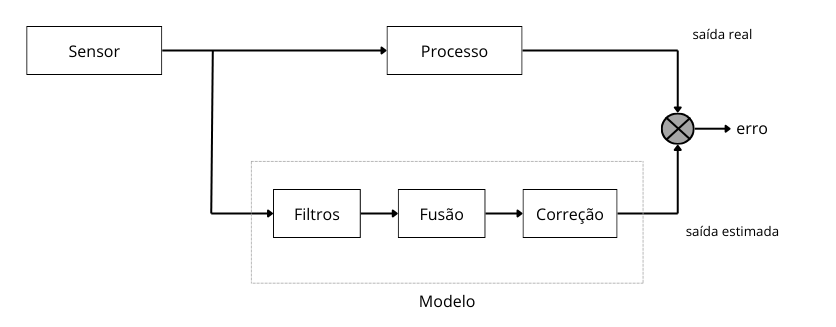
\includegraphics[width=.9\linewidth]{imagens/diagrama.png}
            
            \label{fig:diagrama__}
            \textbf{Fonte:} Autoria Própria
        \end{figure}
    
        O caminho superior, identificado como "Processo", simula a geração do valor verdadeiro da grandeza física, atuando como o padrão de referência contra o qual o sistema será comparado. O caminho inferior, englobado pelo bloco "Modelo", representa a cadeia de processamento do sistema de medição. Este recebe o sinal bruto do "Sensor"\ e aplica etapas de tratamento, incluindo "Filtros", "Fusão"\ de dados e, crucialmente, a "Correção".

        A etapa de "Correção"\ é o ponto onde os coeficientes de calibração, determinados pela análise do "erro"\ resultante da comparação, são aplicados para ajustar a saída do sistema. Portanto, o objetivo da calibração é minimizar o "Erro"\ indicado na saída do comparador, ajustando os parâmetros do bloco de "Correção"\ para que a "Saída Artificial"\ se aproxime ao máximo da "Saída Ideal".

        Diante do exposto, a metodologia descrita, que fundamenta a minimização do erro através do ajuste dos parâmetros de correção, será aplicada experimentalmente utilizando um pêndulo simples como padrão de referência para gerar os valores teóricos esperados. Essa escolha de referência justifica-se pela possibilidade de prever teoricamente o comportamento oscilatório do sistema, permitindo a comparação direta entre os valores medidos pelos sensores e os esperados pelas equações do movimento \cite{cengiz_tepe_6c077d55}.

    \subsection{Pêndulo Simples}
        O instrumento que se utilizará para calibrar o sensor será um pêndulo simples, inspirado no aparato de testes desenvolvido por House \citeyear{thomas_house_1f782b5b}, no qual um pêndulo de 4 metros de comprimento (Figura\autoref{fig:pendulo}), com junta universal de dois graus de liberdade acoplada a encoders angulares e suportado por uma estrutura de quatro pernas similar a um tripé, permitiu a comparação simultânea e direta do desempenho de oito unidades de medição inercial fixadas em uma plataforma balanceada na extremidade inferior do braço. Esse arranjo fornece um movimento oscilatório controlado e matematicamente previsível, no qual o sensor é fixado à massa móvel de modo a registrar as variações contínuas de aceleração e velocidade angular durante os ciclos de oscilação, enquanto as equações fundamentais da física clássica fornecem os valores de referência teóricos para o mesmo intervalo de tempo.

        \begin{figure}[H]
            \centering
            \caption{Esquematização do Pêndulo de Calibração}
            
            \subfloat[Diagrama de Corpo Livre]{
                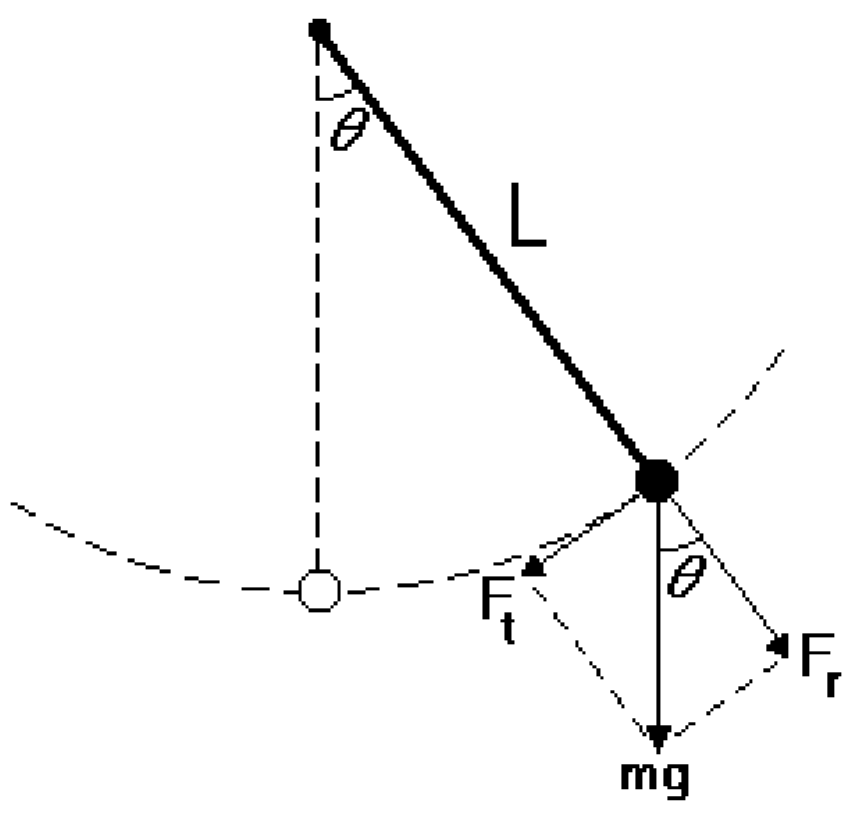
\includegraphics[width=.3\linewidth]{imagens/pendulo1.png}
            }
            \hspace{2cm}
            \subfloat[Ilustração com Dispositivo]{
                \frame{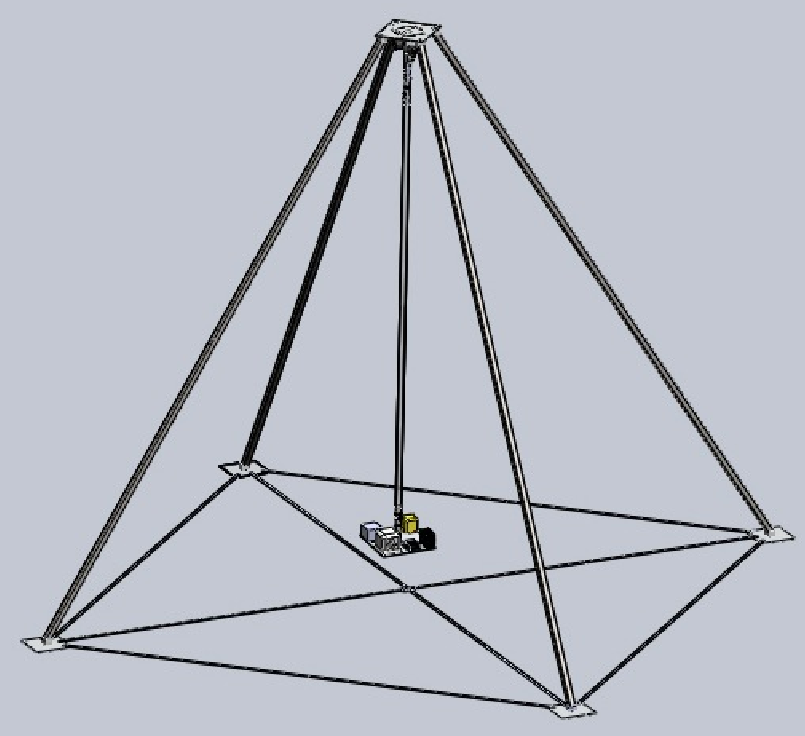
\includegraphics[width=.3\linewidth]{imagens/pendulo2.png}}
            }
            
            \label{fig:pendulo}
            \textbf{Fonte:} \href{https://nrc-publications.canada.ca/eng/view/object/?id=2b49dae2-b5b7-403b-93ba-6b03a40a230b}{House, Thomas}.
        \end{figure}

        O procedimento de calibração pode ser realizado por um método matemático puro ou com instrumentação auxiliar, como encoders discretos de posição angular. Na abordagem matemática, modela-se um pêndulo simples com atrito, decompondo o movimento nos eixos vertical e horizontal. A dinâmica do sistema baseia-se na variação do deslocamento angular $\theta$, cujo coeficiente de atrito $\alpha$ é determinado experimentalmente a partir das oscilações observadas. No entanto, estimativas imprecisas de $\alpha$ podem comprometer a acurácia global do procedimento \cite{mykola_nalisko_ec3a3d96}. Além disso, esse método apresenta um risco de dependência circular, uma vez que o decaimento das oscilações é medido pelo próprio sensor em calibração \cite{warren_w__tryon_a9193008}.

        Diante dos desafios previamente destacados, optou-se pela utilização exclusiva do pêndulo simples equipado com encoder, o qual fornecerá o ângulo de rotação $\theta$ para comparação direta com os dados do sensor. Assim, o dispositivo poderá ser devidamente calibrado ao ser fixado na extremidade inferior do pêndulo e submetido a oscilações em angulações conhecidas. O encoder angular, instalado no eixo de rotação, proporciona a posição exata do braço, viabilizando a comparação entre a leitura de referência e os dados de orientação obtidos pelo sensor inercial \cite{thomas_house_1f782b5b}.

        A estrutura do pêndulo, conforme mostrado na Figura\autoref{fig:desenho_}, foi confeccionada utilizando liga de alumínio 6063-T5, material selecionado por sua relação entre resistência e leveza. A plataforma base, projetada para a fixação dos sensores, é constituída por chapas sobrepostas com dimensões de 400mm x 400mm e 3mm de espessura, integradas a uma estrutura tubular (com diâmetros variando entre 1½” e 2”) que confere robustez ao conjunto. O sistema conta ainda com uma articulação traseira macho e fêmea projetada para acoplamento a um cilindro pneumático (ISO Ø 32mm), assegurando a repetibilidade dos movimentos oscilatórios, e uma chapa superior de dimensões 6,35mm x 200mm x 200mm que permite que o aparato seja fixado, para a realização dos testes.
        
        \begin{figure}[H]
            \centering
            \caption{Desenho Técnico do Pêndulo de Calibração}
            
            \subfloat[]{
                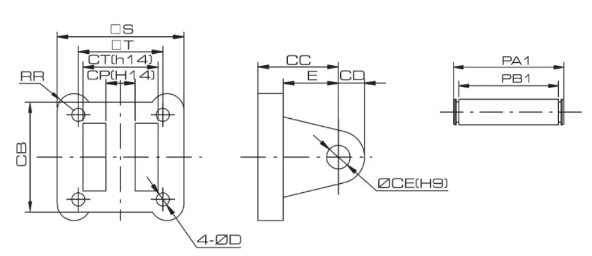
\includegraphics[width=.5\linewidth]{imagens/desenho1.png}
            }
            \subfloat[]{
                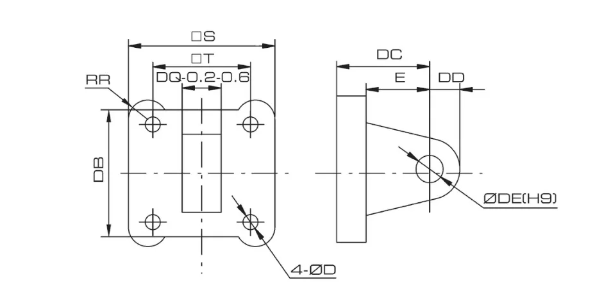
\includegraphics[width=.5\linewidth]{imagens/desenho2.png}
            }
            
            \label{fig:desenho_}
            \textbf{Fonte:} Autoria Própria
        \end{figure}

        A Figura abaixo apresenta a parte superior do aparato, composta por uma chapa superior, tubulação e articulação.

        \begin{figure}[H]
            \centering
            \caption{Chapa Superior do Pêndulo}
        
            \subfloat[]{
                \frame{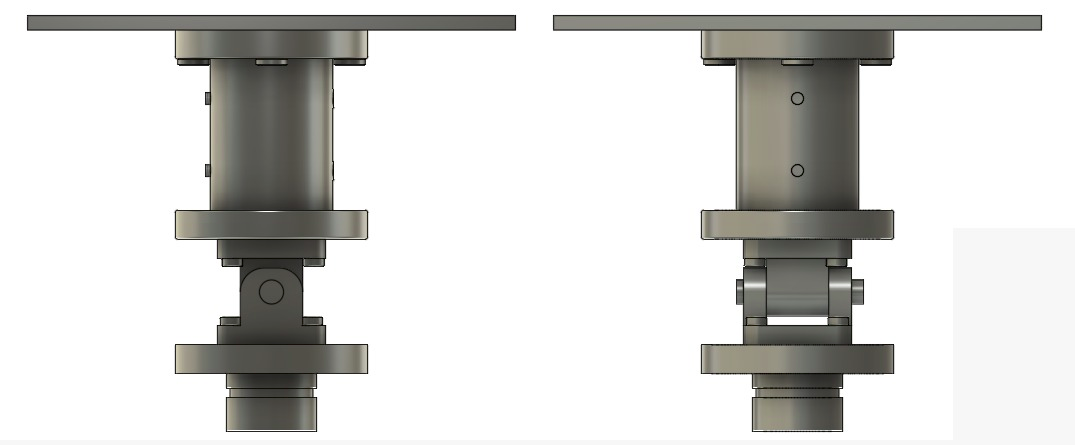
\includegraphics[height=3cm]{imagens/sup2.png}}
            }
            \hspace{1cm}
            \subfloat[]{
                \frame{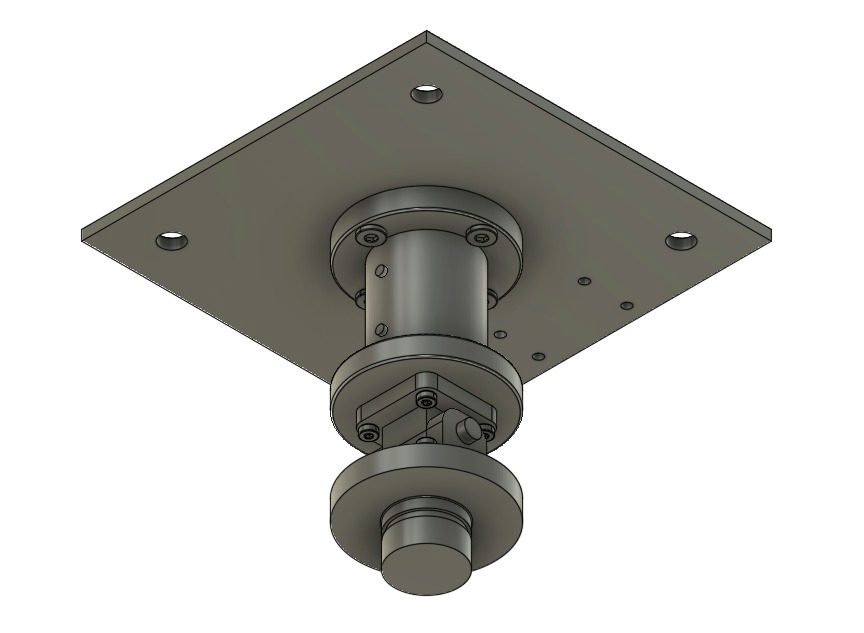
\includegraphics[height=3.3cm]{imagens/sup3.png}}
            }
            
            \label{fig:sup_}
            \textbf{Fonte:} Autoria Própria
        \end{figure}
        
        No que diz respeito à funcionalidade, o Dispositivo de Referência de Movimento (DDRM) permite a rotação da base de fixação, possibilitando a simulação de movimentos tanto no eixo X quanto no eixo Z sem alteração das propriedades físicas do sistema, mantendo a equivalência do período do pêndulo em ambas as orientações. A \autoref{fig:eixo} mostra a orientação descrita devidamente.

         \begin{figure}[H]
            \centering
            \caption{Orientação dos Eixos na Plataforma}
            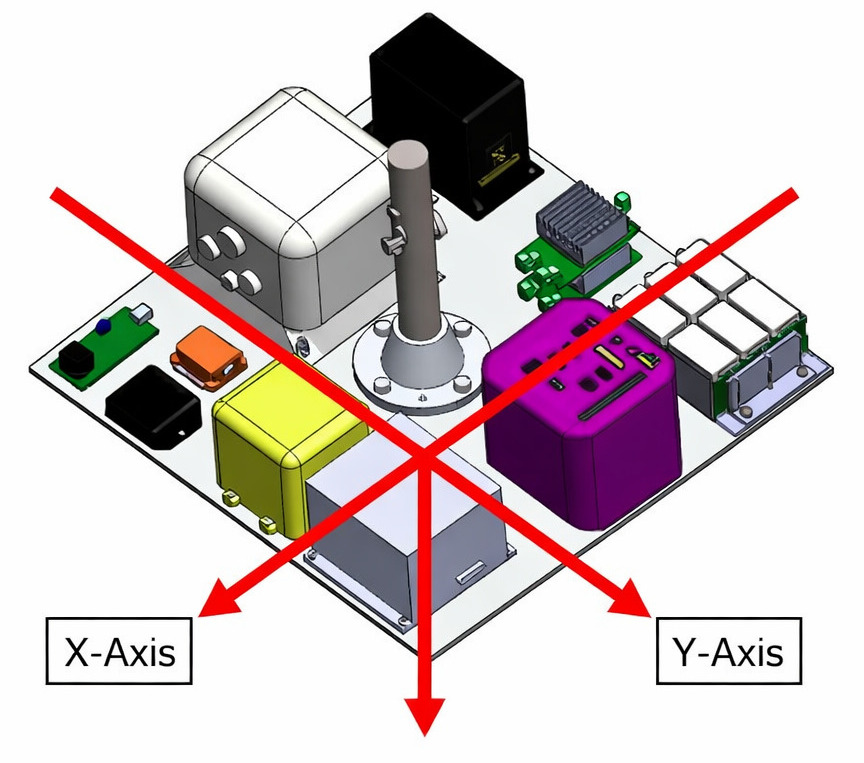
\includegraphics[width=.65\linewidth]{imagens/eixo.png}
            
            \label{fig:eixo}
            \textbf{Fonte:} Fabricante JP MAGNATA
        \end{figure}

        A validação do equipamento e a calibração dos sensores são realizadas através de duas etapas: testes estáticos, destinados à identificação de desvios constantes e estabilidade do sinal; e testes dinâmicos, que avaliam a resposta dos sensores a variações de aceleração e velocidade angular sob diferentes amplitudes de oscilação.

    \subsection{Encoder}
        O encoder é um dispositivo eletromecânico que converte a posição angular de um eixo em pulsos digitais, fornecendo uma medida precisa de referência para calibração de sensores inerciais \cite{cengiz_tepe_6c077d55}. Neste projeto, utiliza-se preliminarmente um modelo comercial E40S6 com resolução de 1024 pulsos por revolução (ppr), equivalente a uma precisão angular de aproximadamente $0,35^\circ$ ($360^\circ / 1024$), selecionado por sua disponibilidade imediata e adequação comprovada em testes experimentais similares com pêndulos. A figura abaixo mostra o encoder que acoplado ao eixo de rotação do pêndulo.

        \begin{figure}[H]
            \centering
            \caption{Encoder Anexado no Pêndulo}
            \frame{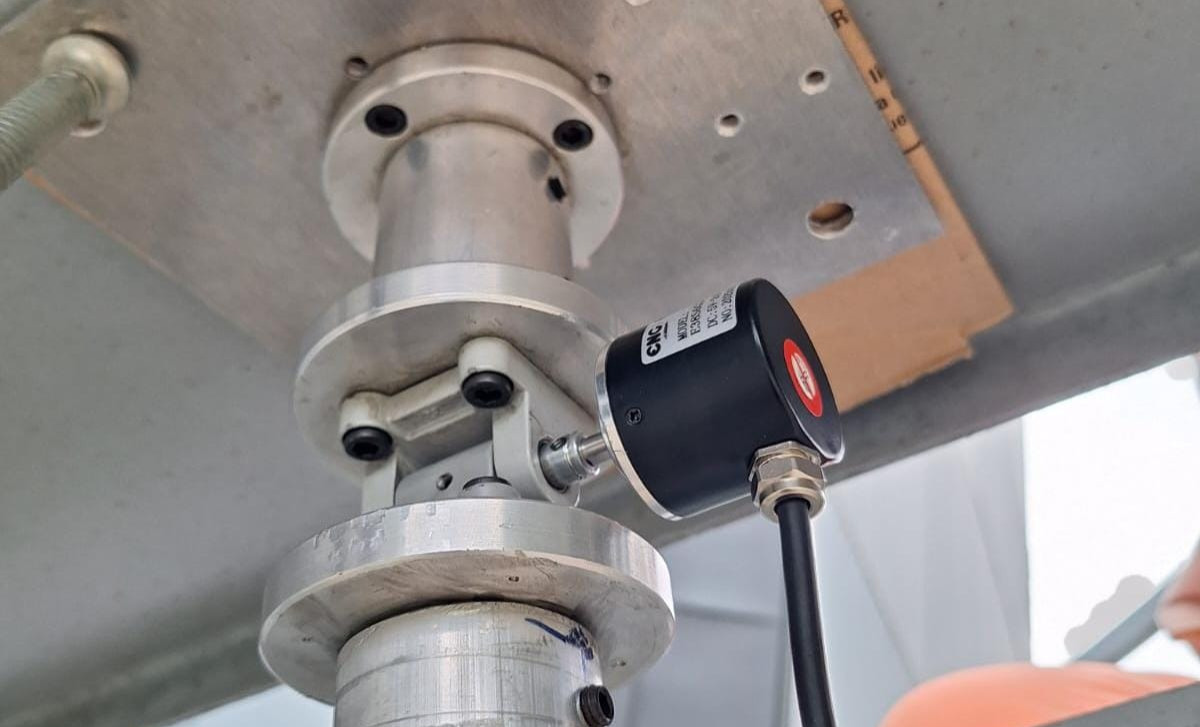
\includegraphics[width=.55\linewidth]{imagens/encoder_.png}}
            
            \label{fig:eixo}
            \textbf{Fonte:} Fabricante JP MAGNATA
        \end{figure}

        Ao rotacionar o pêndulo, o encoder retornará um valor proporcional ao ângulo de rotação, que será comprarado, onde análises comparativas demonstrarão as limitações relativas desse encoder inicial em relação às medições refinadas do sensor Kernel após calibração, destacando a necessidade de um upgrade no dispositivo.
        
    \subsection{Calibração}
        O pêndulo integra uma estrutura tridimensional que possibilita oscilações em ambos os eixos, viabilizando a calibração do sensor inercial. A figura subsequente apresenta o plano cartesiano 3D adotado como referência para o cálculo dos movimentos, derivados do ângulo $\phi$ mensurado pelo encoder, os quais serão comparados aos dados registrados pelo sensor do dispositivo. Assim, o gráfico apresentado na \autoref{fig:graf_stew} ilustra a conversão de coordenadas esféricas para retangulares ao localizar um ponto no espaço 3D \cite{james_stewart_51d108d3}. 
        
        \begin{figure}[H]
            \centering
            \caption{Orientação Utilizada}
            \subfloat[Orientação Cartesiana 3D]{
                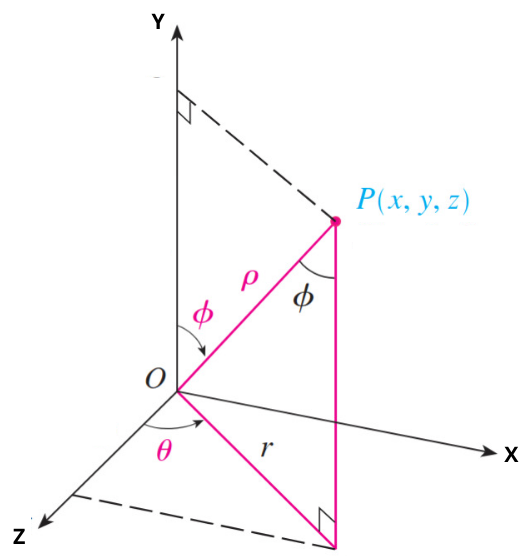
\includegraphics[height=5.5cm]{imagens/graf3d.png}
            }
            \subfloat[Orientação do Sensor Kernel]{
                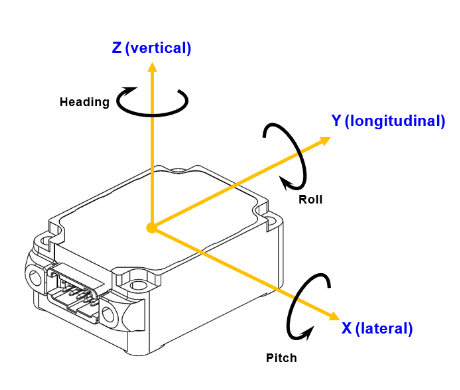
\includegraphics[height=5.5cm]{imagens/kernel2.png}
            }
            \subfloat[Orientação do Sensor Kernel]{
                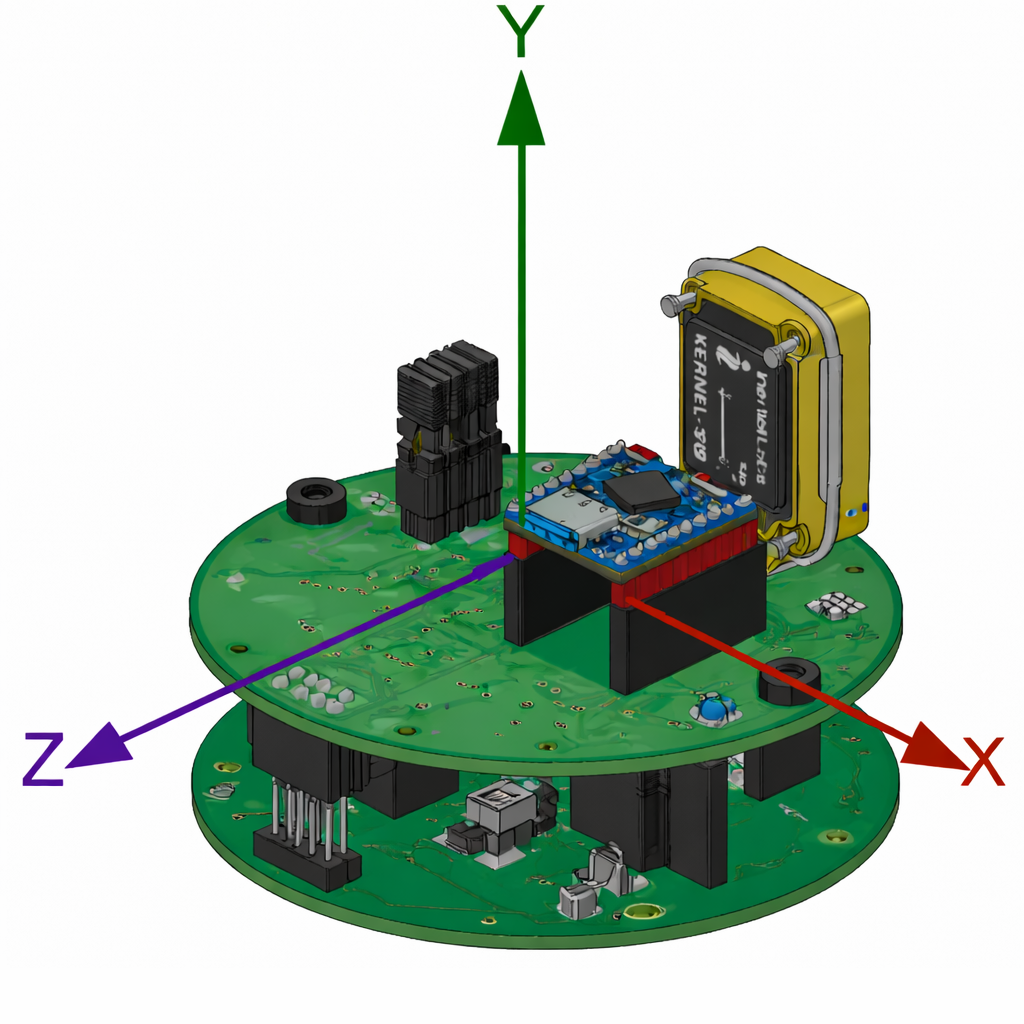
\includegraphics[height=5.5cm]{imagens/kernel3.png}
            }
            
            \label{fig:graf_stew}
            \textbf{Fonte:} Autoria Própria
        \end{figure}


         Nesse sistema de coordenadas, $\rho$ representa a distância da origem, $\phi$ é o ângulo a partir do eixo vertical y, e $\theta$ é o ângulo de rotação no plano horizontal xz. A calibração será feita inferindo a partir de $\phi(t)$ as variáveis que serão comparadas com os dados brutos obtidos a partir do acelerômetro e do giroscópio.

         \subsubsection{Giroscópio}
            Para fins de exemplificação, ao posicionar o pêndulo variando somente o eixo $x$, é possível calibrar a velocidade angular referente ao eixo $x$, uma vez que o eixo $y$ não sofrerá variação. Portanto, o ângulo $\theta$ será constante em $0$º permitindo tratar a calibração de maneira bidimensional, como mostrado na \autoref{fig:2daccel}.

            \begin{figure}[H]
                \centering
                \caption{Representação 2D para Calibração}
                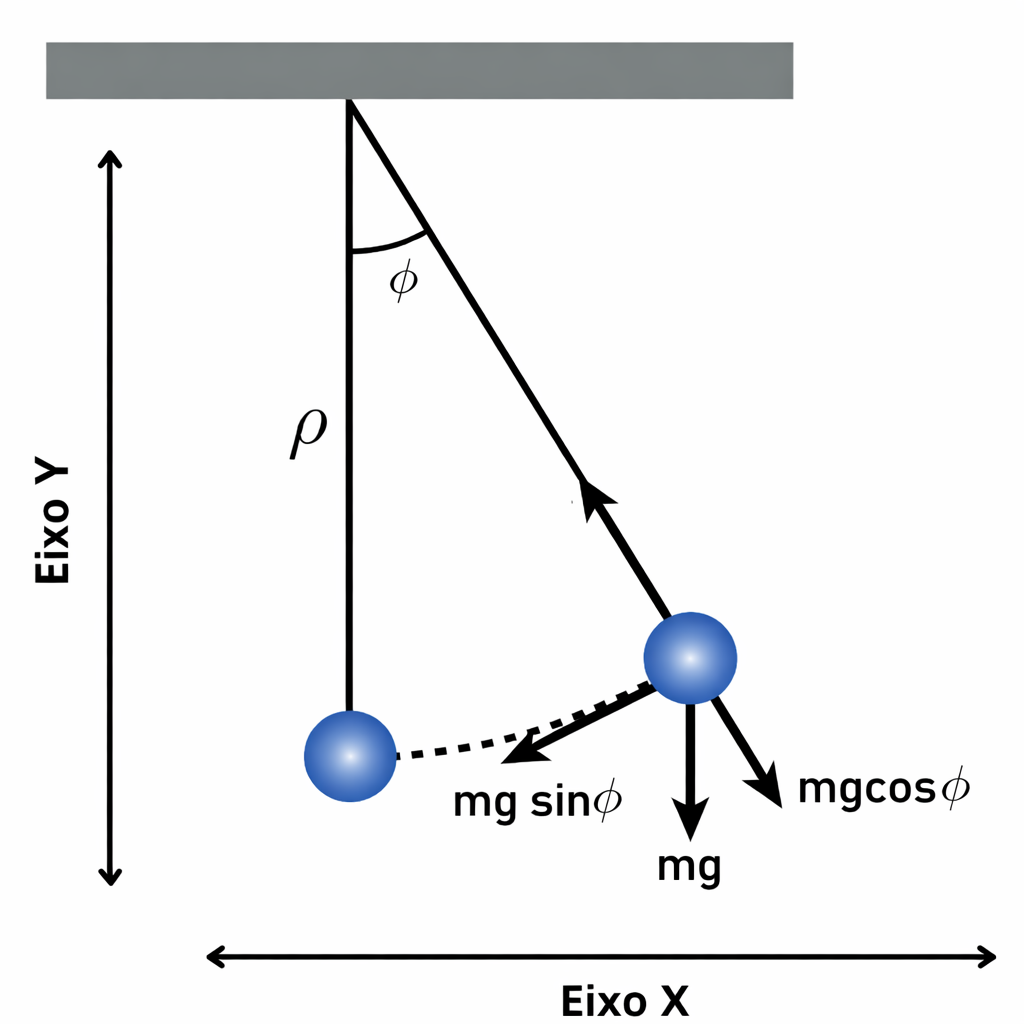
\includegraphics[width=.37\linewidth]{imagens/dsd.png}
                
                \label{fig:2daccel}
                \textbf{Fonte:} Autoria Própria
            \end{figure}

            A velocidade angular pode ser encontrada a partir de derivação simples do ângulo $\phi$, conforme a \autoref{eq:omega}.

            \begin{equation}
                \label{eq:omega}
                \phi'_x(t) = \frac{d\phi}{dt}
            \end{equation}

            Dessa forma, o ângulo de referência $\phi(t)$ deve ser sincronizado no tempo com os dados brutos do giroscópio e acelerômetro do sensor $\phi_s(t)$ e $a_s(t)$, onde o eixo a ser variado será calibrado e ajustado por meio de uma função linear simples, dada por:

            \begin{equation}
                \phi(t) = A\cdot\phi_s(t) + B  
                \text{\hspace{.7cm}e\hspace{.7cm}} 
                \phi'(t) = C\cdot\phi'_s(t) + D
            \end{equation}

            Através do método dos Mínimos Quadrados Ordinários (OLS), o algoritmo extrai os parâmetros intrínsecos do hardware. Os fatores de escala $B$ e $D$, corrigem a sensibilidade proporcional do sensor, e o viés (Bias), que compensa o erro de deslocamento do sinal quando o dispositivo se encontra em repouso. A eficácia desse ajuste é posteriormente avaliada por métricas de erro absoluto, como o RMSE (Root Mean Square Error).

        \subsubsection{Acelerômetro}
            Diferentemente do giroscópio, a aferição do acelerômetro acoplado à extremidade do pêndulo é governada por uma dinâmica altamente não-linear. O sensor registra a força específica no referencial local da sua carcaça (solidário ao movimento), o que significa que ele sofre a influência simultânea da aceleração tangencial, da aceleração centrípeta e da decomposição vetorial contínua da gravidade em seus eixos devido à inclinação variante. Assim, é possível inferir tais variáveis a partir do encoder com ângulo $\phi(t)$ a partir das equações:

            \begin{equation}
                a_x(t) = \rho\cdot\phi''+g\cdot sin(\phi)
                \text{\hspace{.7cm}e\hspace{.7cm}} 
                a_y(t) = \rho\cdot\phi'^2+g\cdot cos(\phi)
            \end{equation}

            Na equação do eixo $x$, o termo $\rho\cdot\phi''$ isola a componente tangencial do movimento, enquanto $g\cdot sin(\phi)$ rastreia a projeção variante da gravidade. De forma análoga, no eixo $z$, a não-linearidade é capturada pelo comportamento quadrático da força centrípeta $\rho\cdot\phi'^2$ e pelo cosseno da gravidade. A calibração é feita de forma identica ao giroscópio comparando linearmente a variável de referência à variável do sensor, como mostrado na \autoref{eq:accel}.

            \begin{equation}
                \label{eq:accel}
                a_x(t) = A\cdot a_{xs}(t) + B  
                \text{\hspace{.7cm}e\hspace{.7cm}} 
                a_y(t) = C\cdot a_{ys}(t) + D
            \end{equation}

            Da mesma forma como seria a calibrção variando o eixo $x$, a calibração do eixo $z$ consistiriam nas mesmas fórmulas, finalizando assim a metodologia.
        
        
\newpage
\section{Desenvolvimento}
    O dispositivo desenvolvido é equipado com um processador ESP32-S3 Mini de alto desempenho, dual-core Xtensa LX7 com clock de até 240 MHz e suporte nativo a WiFi e Bluetooth, integrado a uma placa de circuito impresso personalizada, juntamente com o sensor de orientação Kernel Motion Sensor AHRS (6/9 graus de liberdade), que proporciona medições precisas de aceleração linear, velocidade angular e orientação com ruído mínimo e filtragem embarcada. Todo o sistema embarcado é abrigado em uma embalagem protetora projetada em CAD e manufaturada por impressão 3D em material ABS de alta resistência mecânica, assegurando proteção ambiental, ergonomia para fixação no pêndulo de calibração e massa otimizada (451,6 g), inferior à de equipamentos comerciais equivalentes.

    \subsection{Testes de Bancada}
        O protótipo do dispositivo de monitoramento, evidenciado nas figuras subsequentes, mostra-se preparado para análises e testes experimentais. Conforme detalhado na metodologia, seus dados serão coletados por um computador e separados para futura análise. O microcontrolador alcança a frequência de amostragem de 100 Hz enviando dados de orientação em tempo real ao respectivo receptor através da comunicação estabelecida. A \autoref{fig:montado} mostra o processo de captura e o armazenamento local dos dados do sensor pelo computador.

        \begin{figure}[H]
            \centering
            \caption{Extração de Dados em Bancada}
            \frame{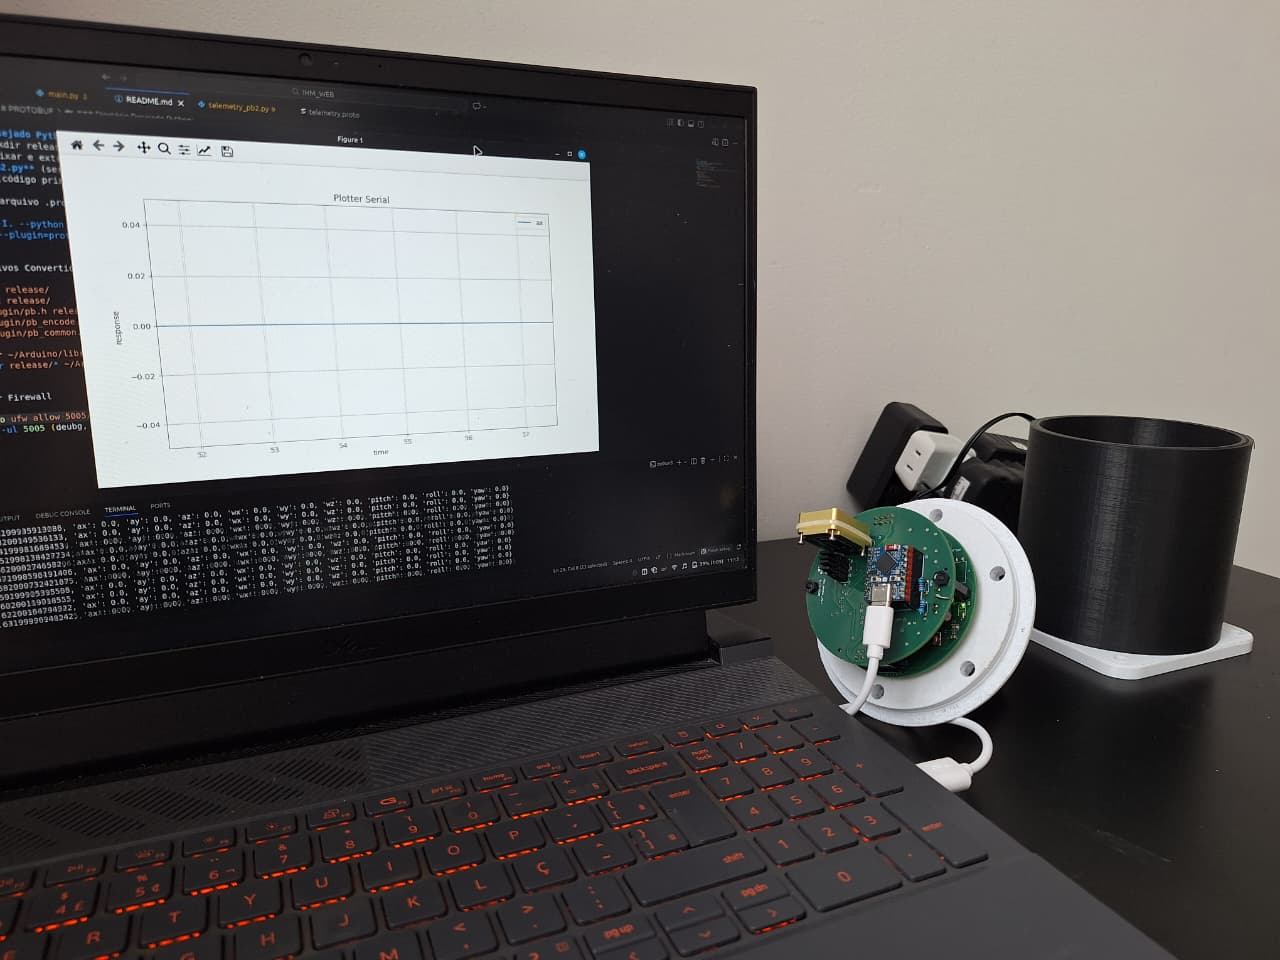
\includegraphics[width=.65\linewidth]{imagens/montado.png}}
            
            \label{fig:montado}
            \textbf{Fonte:} Autoria Própria
        \end{figure}

        A transmissão dessas informações pode ocorrer tanto por conexão física, via porta USB ou cabo RS422 com conversor, quanto remotamente, por meio de rede Wi-Fi. Na modalidade sem fio, utiliza-se o Protocol Buffers, tecnologia desenvolvida pela Google para serialização eficiente de dados estruturados em formato binário compacto \cite{samuel_jackson_57e74ab7}, que otimiza o envio contínuo de informações, garantindo alta velocidade de comunicação e maior praticidade ao eliminar a necessidade de cabos durante os testes. Ambas as modalidades asseguram a integridade da coleta de dados e operam em frequências configuráveis de até 100 Hz.

        Com o funcionamento do protótipo validado na placa de circuito impresso, a etapa seguinte consistiu na integração do sistema embarcado ao compartimento projetado na plataforma Fusion 360 e manufaturado via impressão 3D. A versão preliminar da caixa (Figura\autoref{fig:modelagem_}), objetiva a análise dimensional e ergonômica, permitindo verificar o acoplamento dos componentes, a necessidade de ajustes na altura dos pinos de fixação e a adequação dos orifícios para os parafusos responsáveis pelo fechamento do conjunto. A caixa contém o logotipo do Instituto Federal Fluminense (IFF) na tampa superior, conforme detalhado na modelagem tridimensional da macroentrega anterior, sendo a vedação do estojo garantida pela aplicação de seis parafusos com porcas para fixação.
        
        \begin{figure}[H]
            \centering
            \caption{Dispositivo na Embalagem 1.0}
            
            \subfloat[Partes Desmontadas]{
                \frame{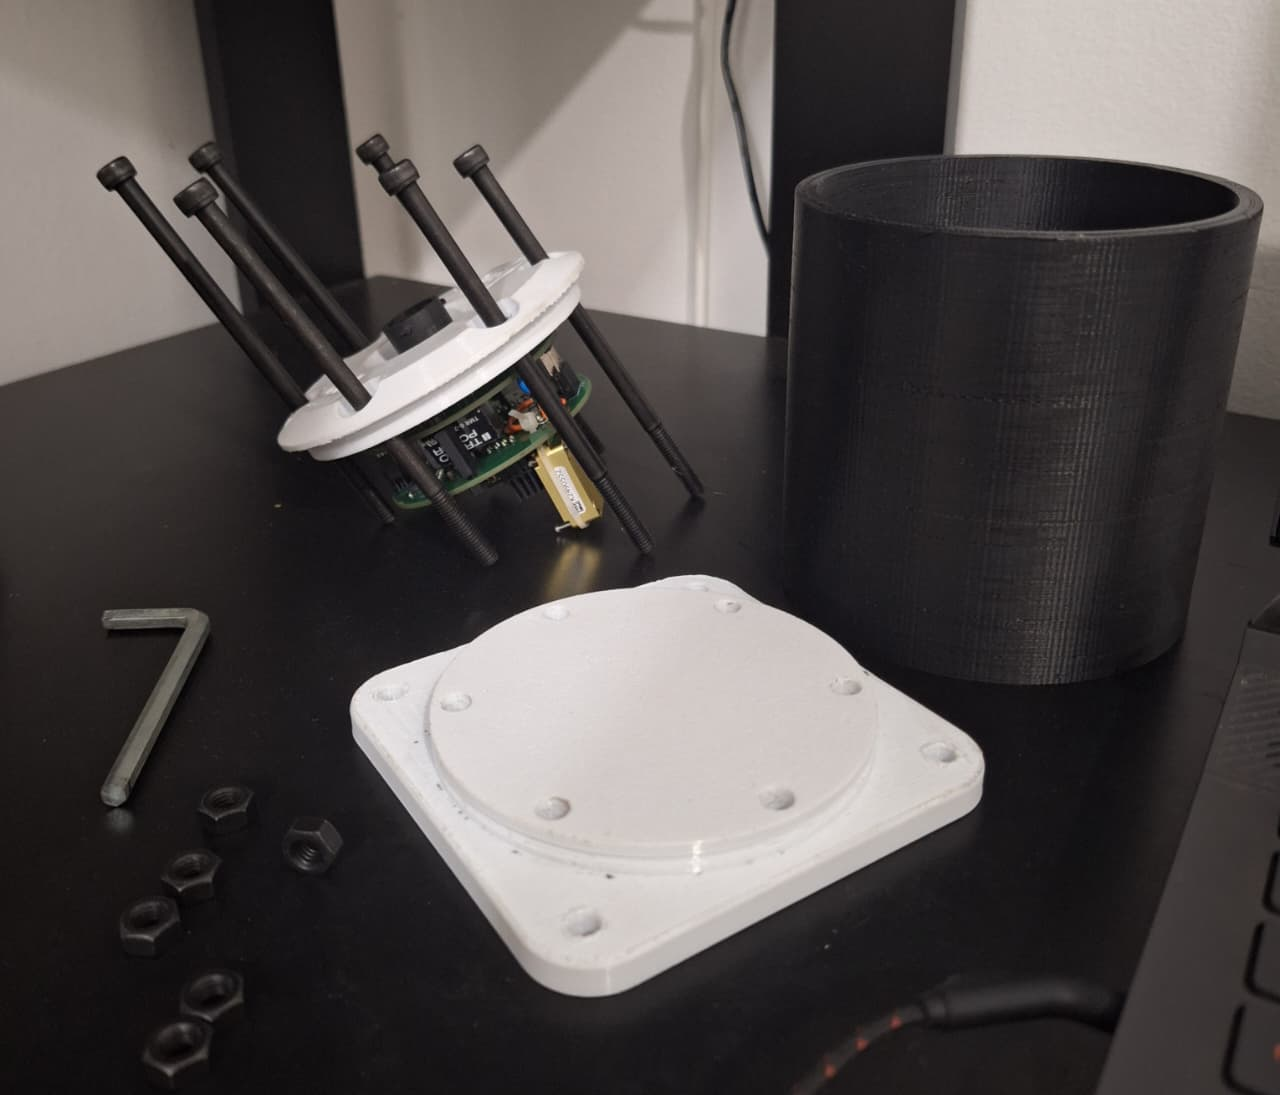
\includegraphics[height=5.6cm]{imagens/modelagem_1.jpeg}}
            }
            \hfill
            \subfloat[Tampa Superior]{
                \frame{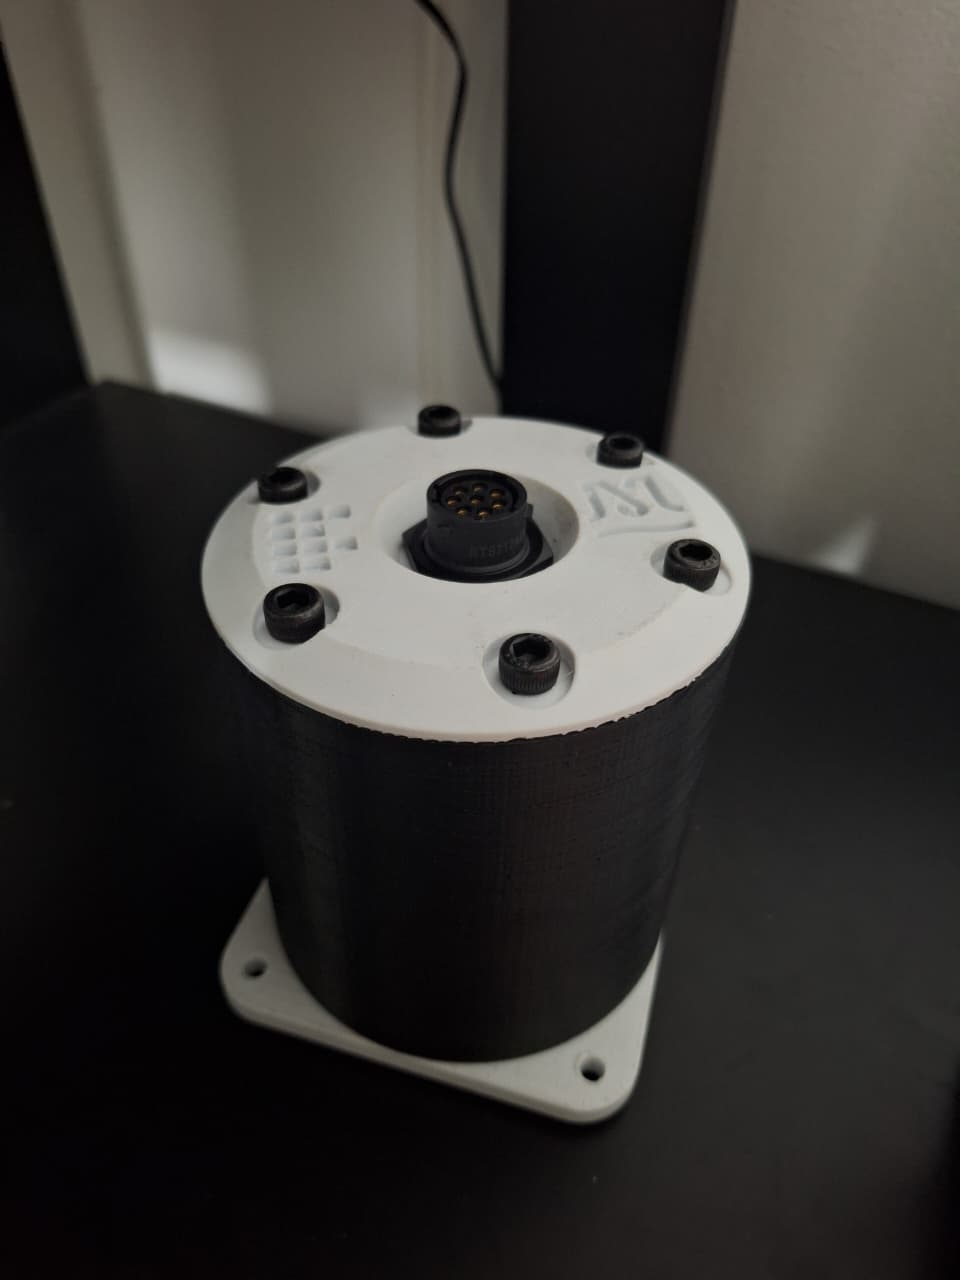
\includegraphics[height=5.6cm]{imagens/modelagem_2.jpeg}}
            }
            \hfill
            \subfloat[Sistema Embarcado]{
                \frame{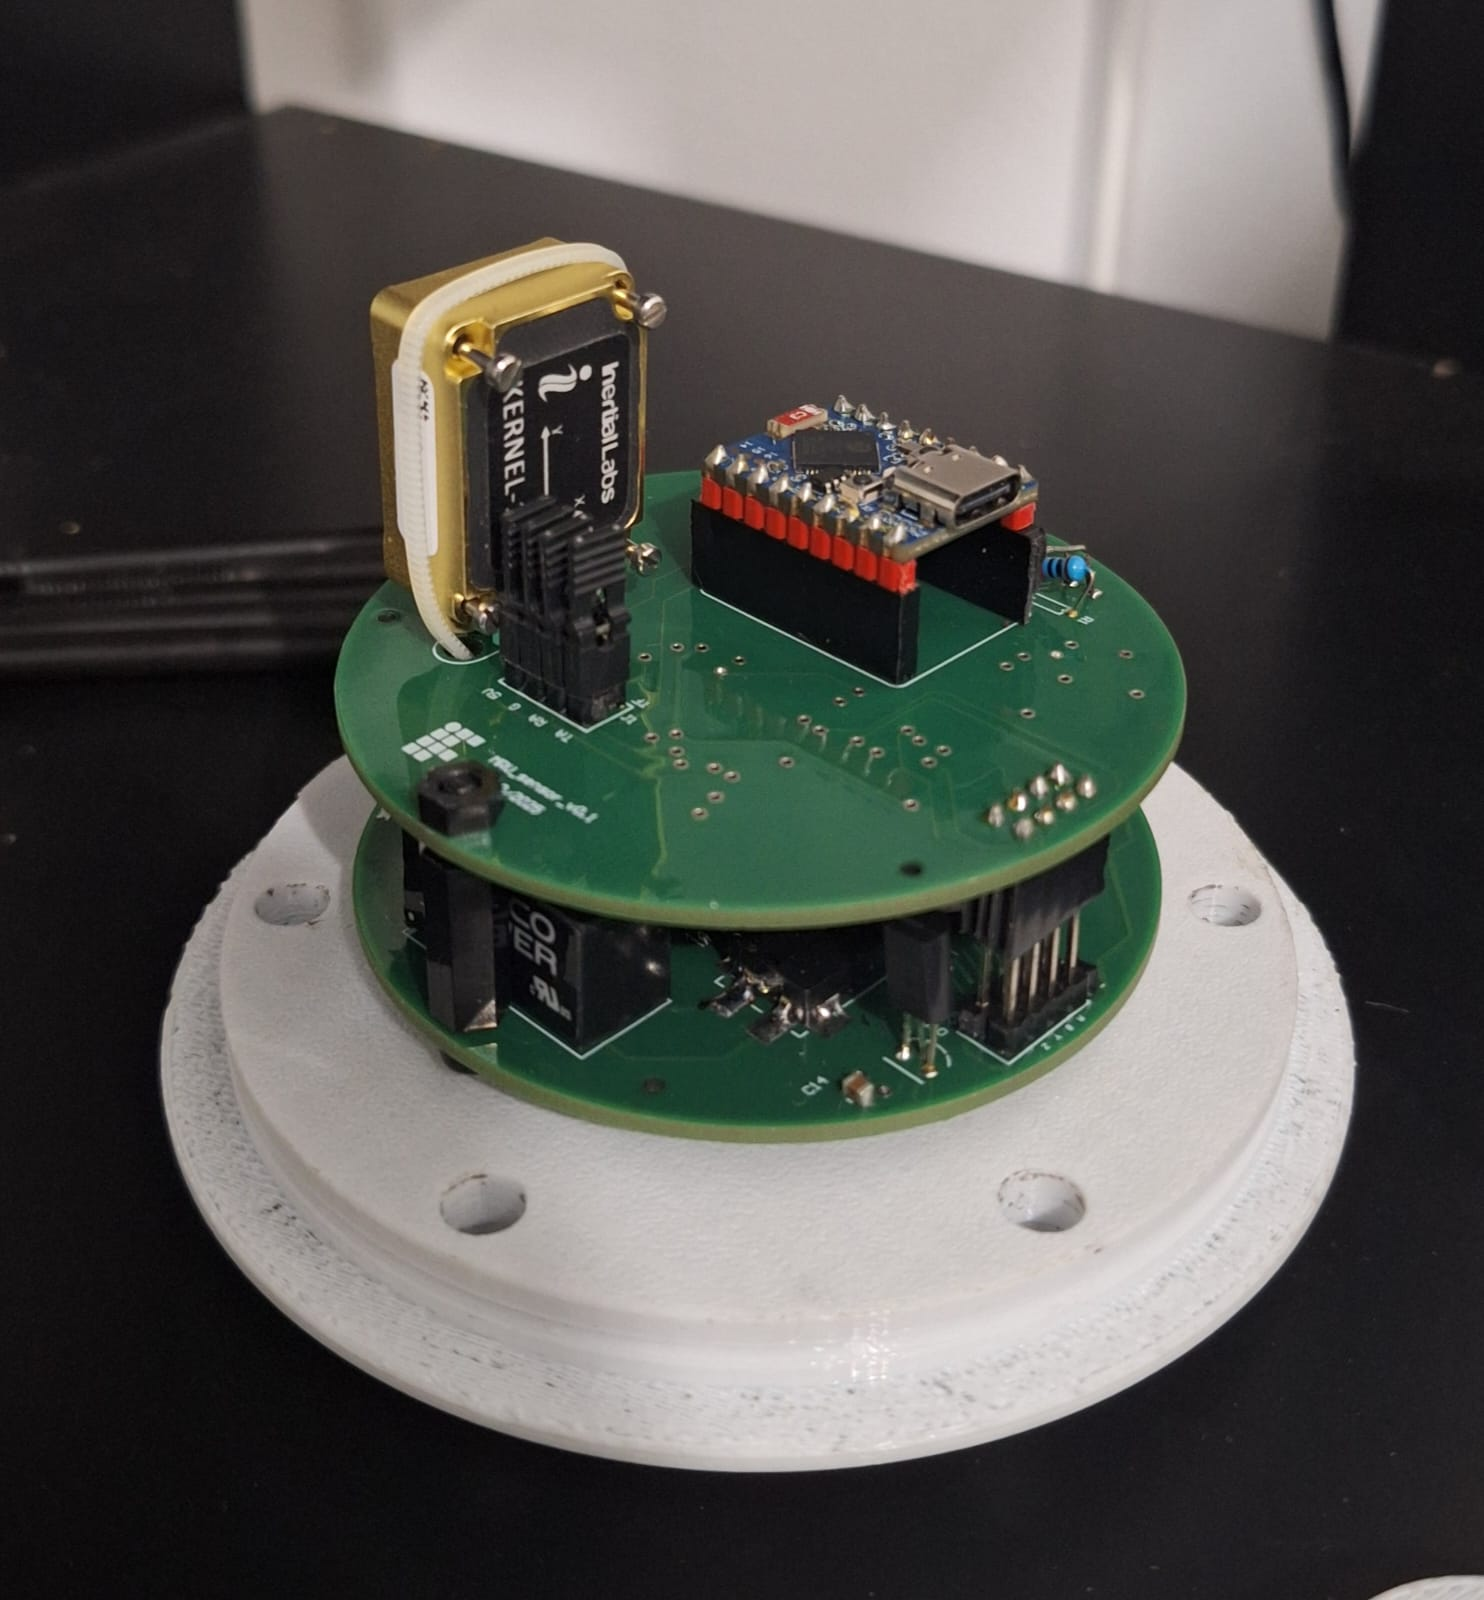
\includegraphics[height=5.6cm]{imagens/modelagem_3.jpeg}}
            }
            
            \label{fig:modelagem_}
            \textbf{Fonte:} Autoria Própria
        \end{figure}
        
        A segunda versão do compartimento, apresentada na Figura\autoref{fig:compartimento_}, foi manufaturada na cor preta para conferir maior sobriedade e acabamento profissional ao protótipo, além de apresentar as correções dimensionais necessárias identificadas na etapa anterior. O sistema embarcado foi acomodado integralmente no interior da estrutura e fixado com parafusos, sem intercorrências na montagem, o que valida as modificações geométricas realizadas. A conexão física ocorre através de um orifício cilíndrico na parte superior, destinado ao cabo de alimentação que também viabiliza a comunicação serial para configuração e extração de dados via computador, embora o dispositivo mantenha a funcionalidade de transmissão sem fio detalhada previamente.

        \begin{figure}[H]
            \centering
            \caption{Dispositivo na Embalagem 2.0}
            
            \subfloat[]{
                \frame{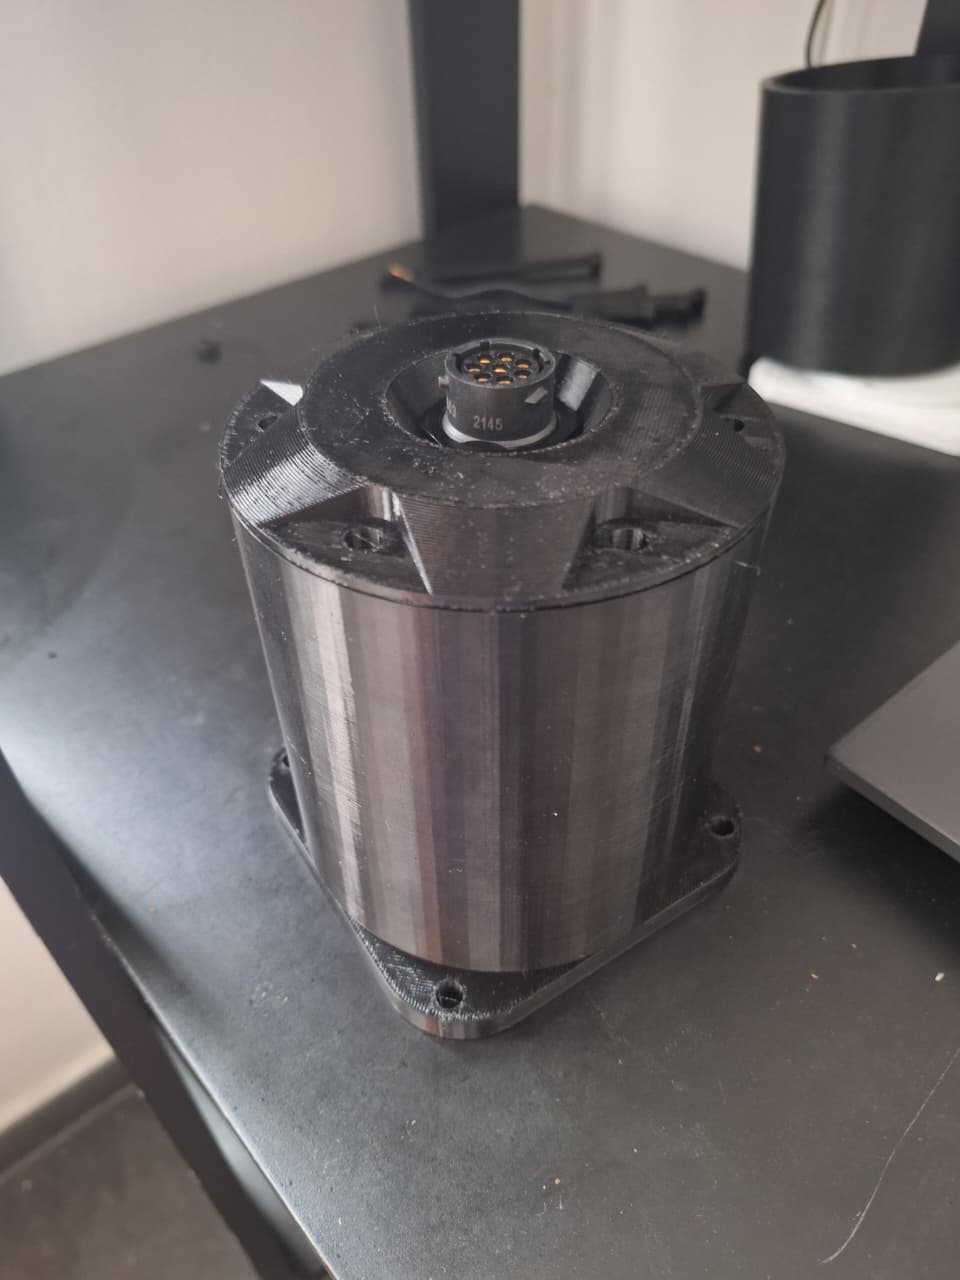
\includegraphics[height=7cm]{imagens/prot_mont_1.png}}
            }
            \hfill
            \subfloat[]{
                \frame{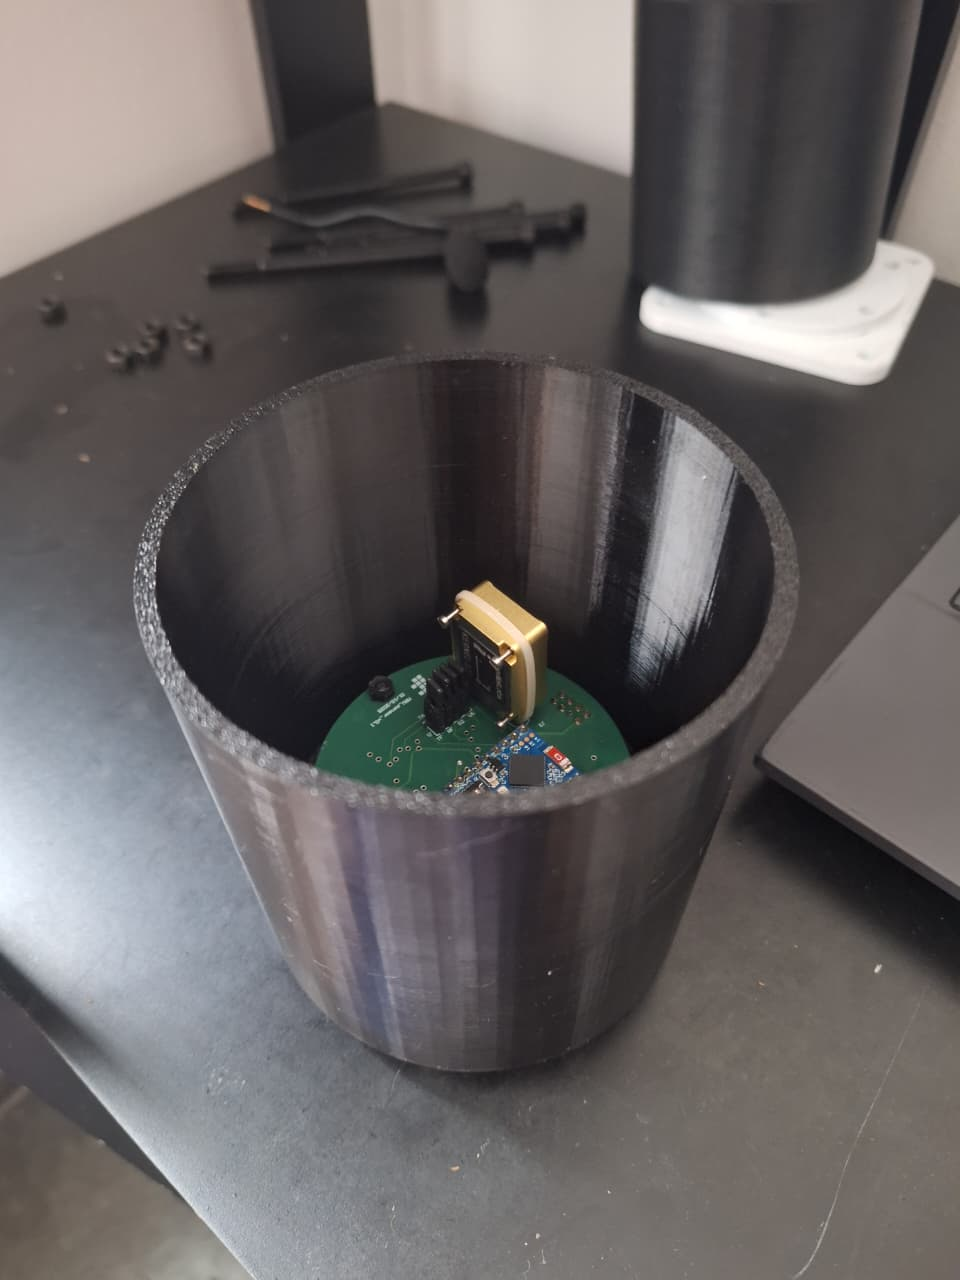
\includegraphics[height=7cm]{imagens/prot_mont_2.png}}
            }
            \hfill
            \subfloat[]{
                \frame{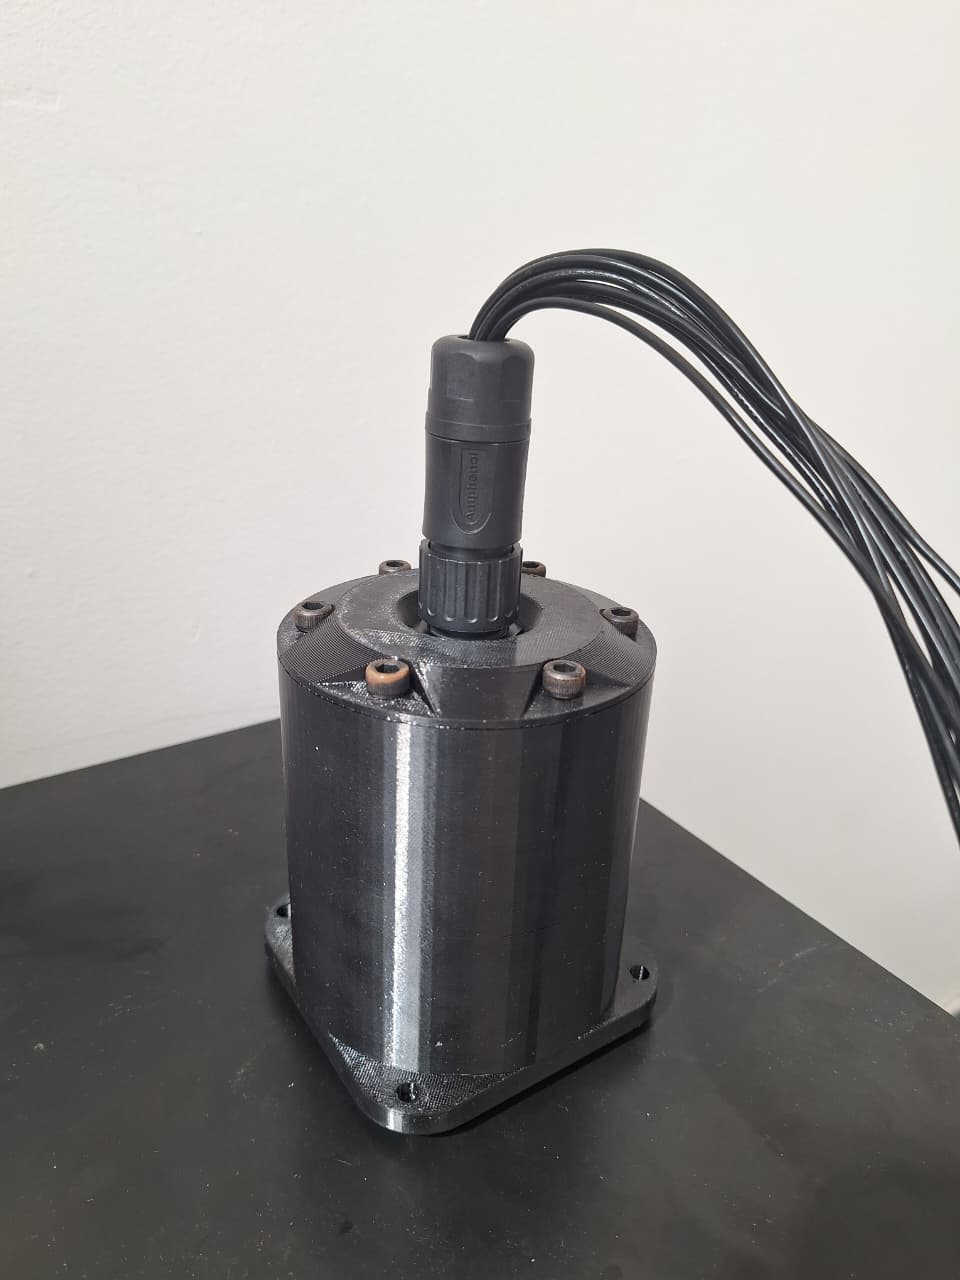
\includegraphics[height=7cm]{imagens/prot_mont_3.png}}
            }
            
            \label{fig:compartimento_}
            \textbf{Fonte:} Autoria Própria
        \end{figure}

        A aferição da massa do dispositivo, realizada com uma balança de precisão após o selamento no novo compartimento, resultou em um valor total de 451,6 g, conforme ilustrado na \autoref{fig:balanca}. Tal medida apresenta-se inferior à dos equipamentos concorrentes, o que se justifica pela ausência, nesta etapa do projeto, de revestimentos metálicos baseados em ligas de cobre e chumbo, materiais comumente utilizados no mercado para blindagem. Este dado atual serve como um parâmetro inicial fundamental para futuras comparações e adequações estruturais.
       
       \begin{figure}[H]
            \centering
            \caption{Dispositivo Pesado em uma Balança de Precisão}
            \frame{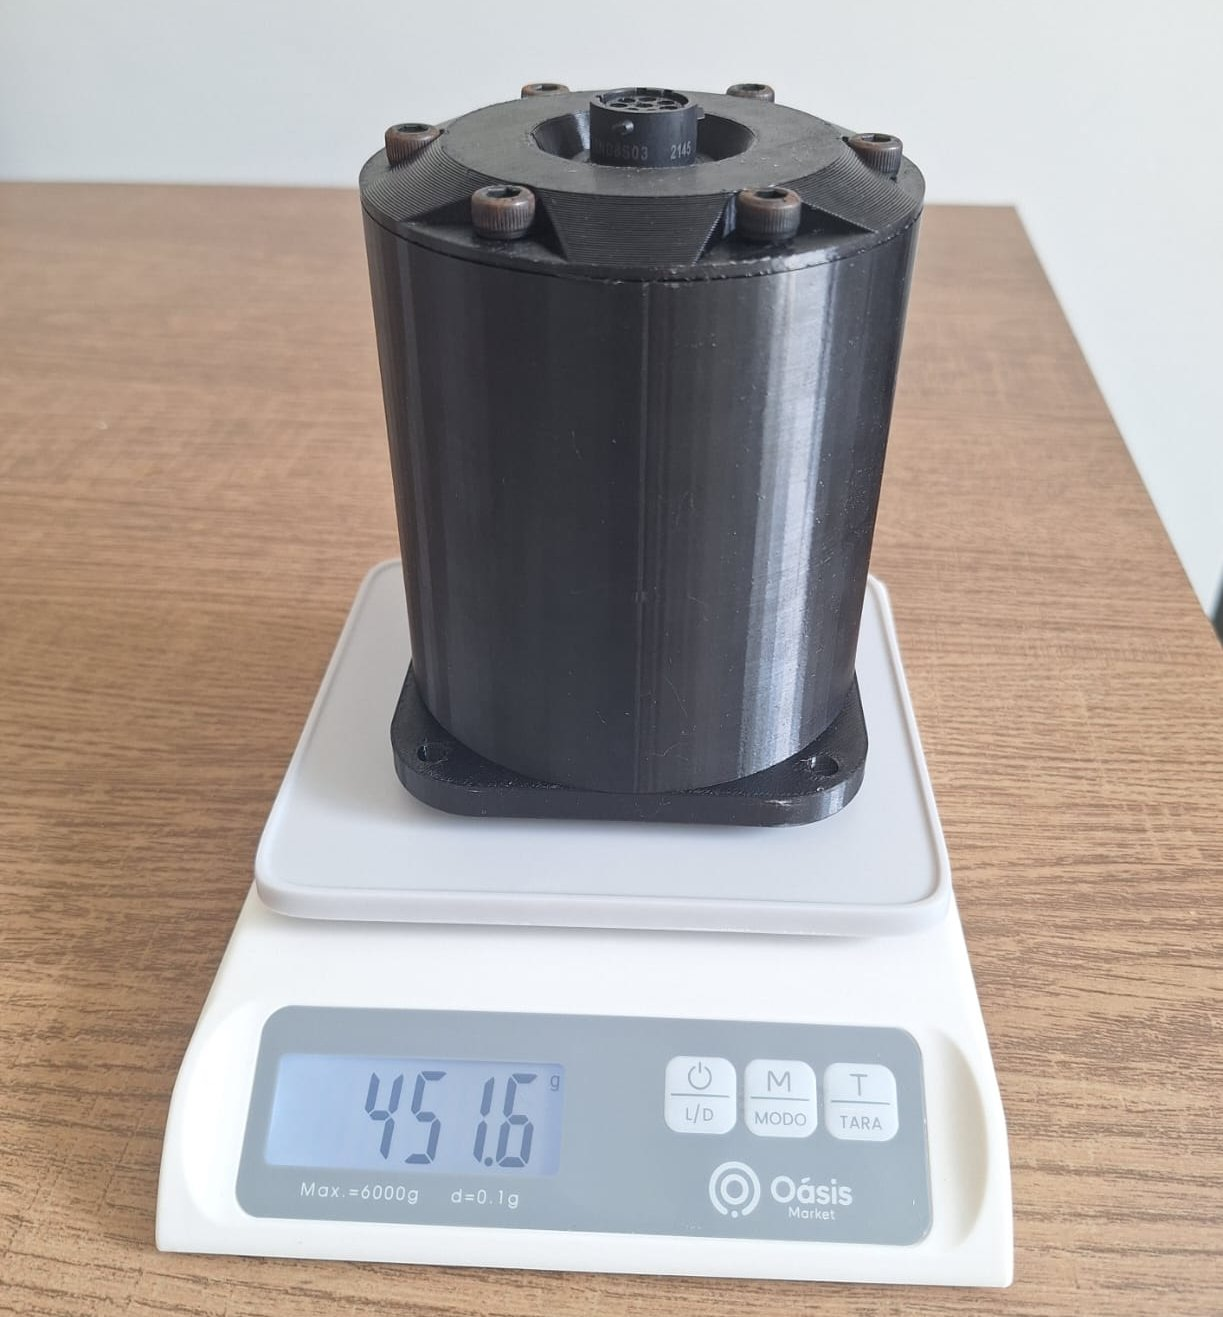
\includegraphics[width=0.4\linewidth]{imagens/balanca.jpeg}}
            
            \label{fig:balanca}
            \textbf{Fonte:} Autoria Própria
        \end{figure}

    \subsection{Montagem do Pêndulo}
        O pêndulo simples, descrito na seção de metodologia, foi implementado conforme as especificações apresentadas e pode ser visualizado na figura subsequente. Ele foi montado e posicionado de forma adequada para possibilitar rotação contínua e fluida em um eixo específico. Inicialmente, posicionou-se o conjunto em uma escada, fixado na parte superior com apenas uma haste, permitindo oscilação livre para coleta de dados que capturassem o comportamento do pêndulo e iniciassem os algoritmos iniciais de calibração.

        \begin{figure}[H]
            \centering
            \caption{Pêndulo Montado em Testes de Bancada}
            
            \subfloat[]{
                \frame{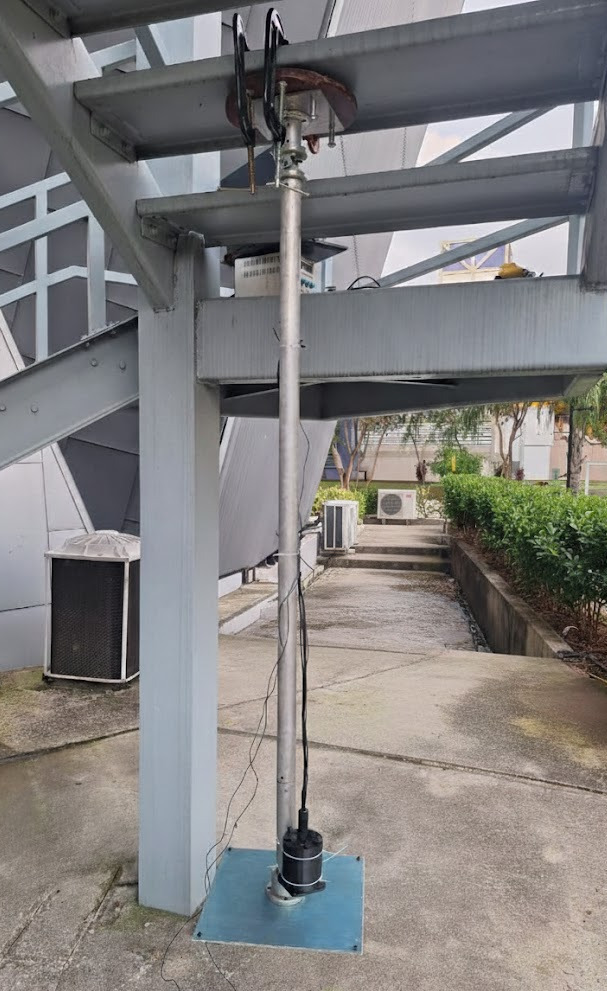
\includegraphics[height=11cm]{imagens/pmont1.png}}
            }
            \hspace{1cm}
            \subfloat[]{
                \frame{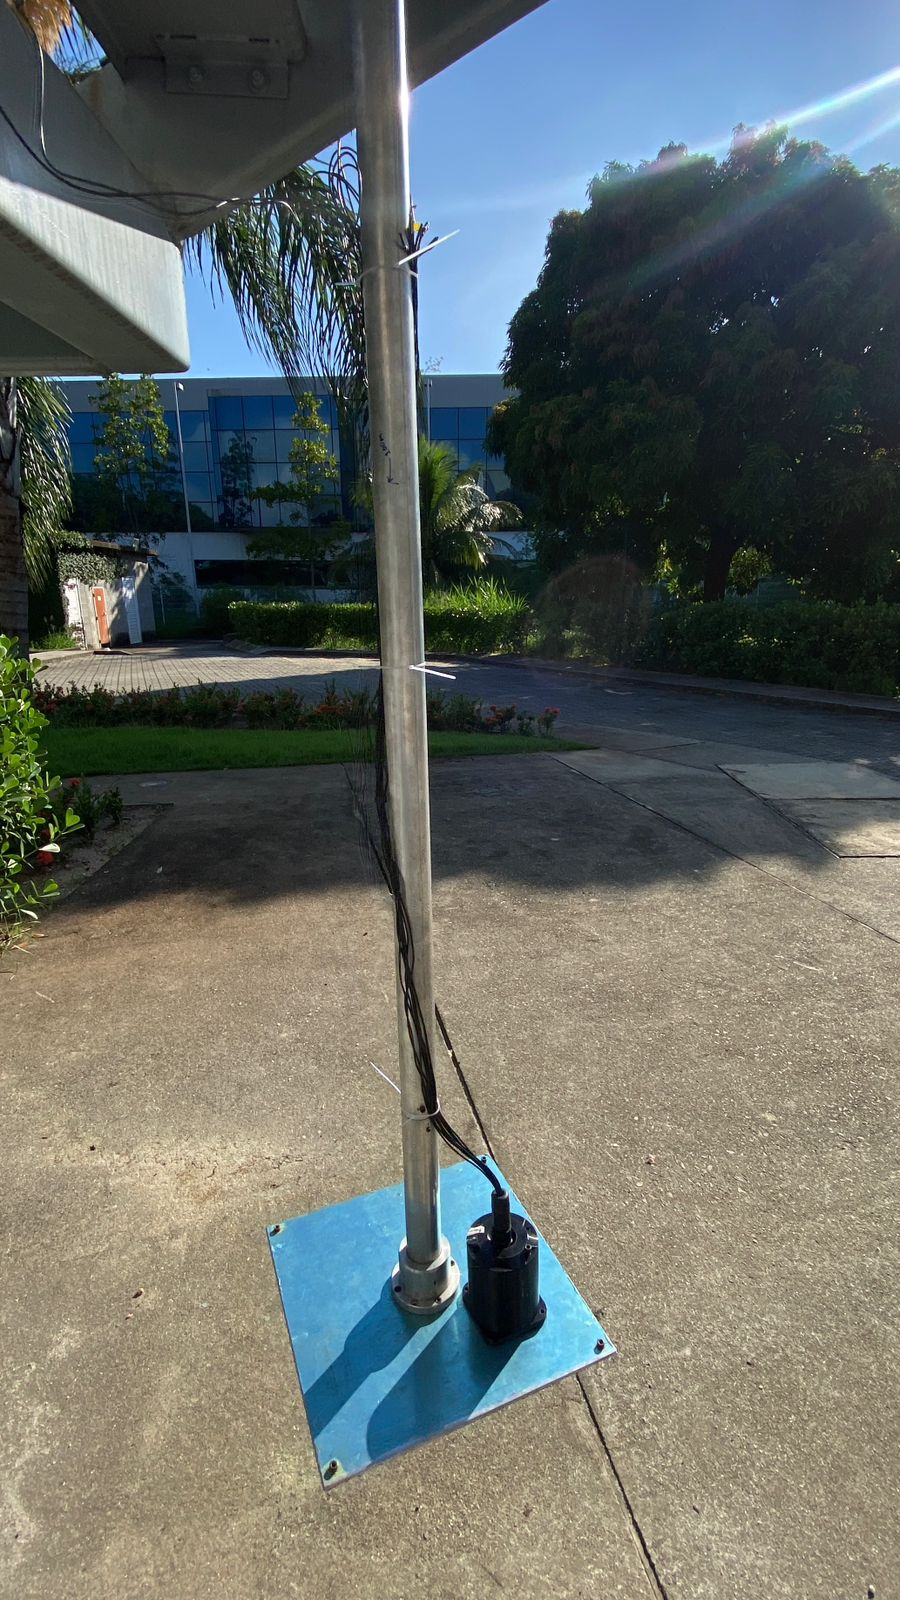
\includegraphics[height=11cm]{imagens/pmont3.png}}
            }
            
            \label{fig:compartimento_}
            \textbf{Fonte:} Autoria Própria
        \end{figure}

        O dispositivo de monitoramento foi fixado na extremidade inferior do pêndulo simples, com seus dados inicialmente transmitidos, juntamente com os obtidos pelo encoder, via streaming Protocol Buffers para um computador responsável pela coleta e armazenamento em arquivos CSV. Essas informações serão analisadas graficamente e matematicamente nas seções subsequentes.
        
        
    \newpage
    \subsection{Testes Estáticos e Dinâmicos com DRMM}
       Com o dispositivo configurado e validado, procedeu-se à execução de sua função primordial de monitoramento de movimento mediante a coleta das variáveis de interesse, nomeadamente a aceleração linear e a velocidade angular nos três eixos cartesianos, bem como as variáveis de orientação Pitch, Roll e Yaw. Os dados foram obtidos utilizando a estrutura previamente detalhada e o comportamento dinâmico do sistema é apresentado na \autoref{fig:graphs}, na qual o eixo das abscissas representa o tempo e o eixo das ordenadas indica a magnitude da respectiva variável de movimento monitorada.
       
         \begin{figure}[H]
            \centering
            \caption{Orientação Gráfica de Todas as Variáveis do Sensor Kernel}
            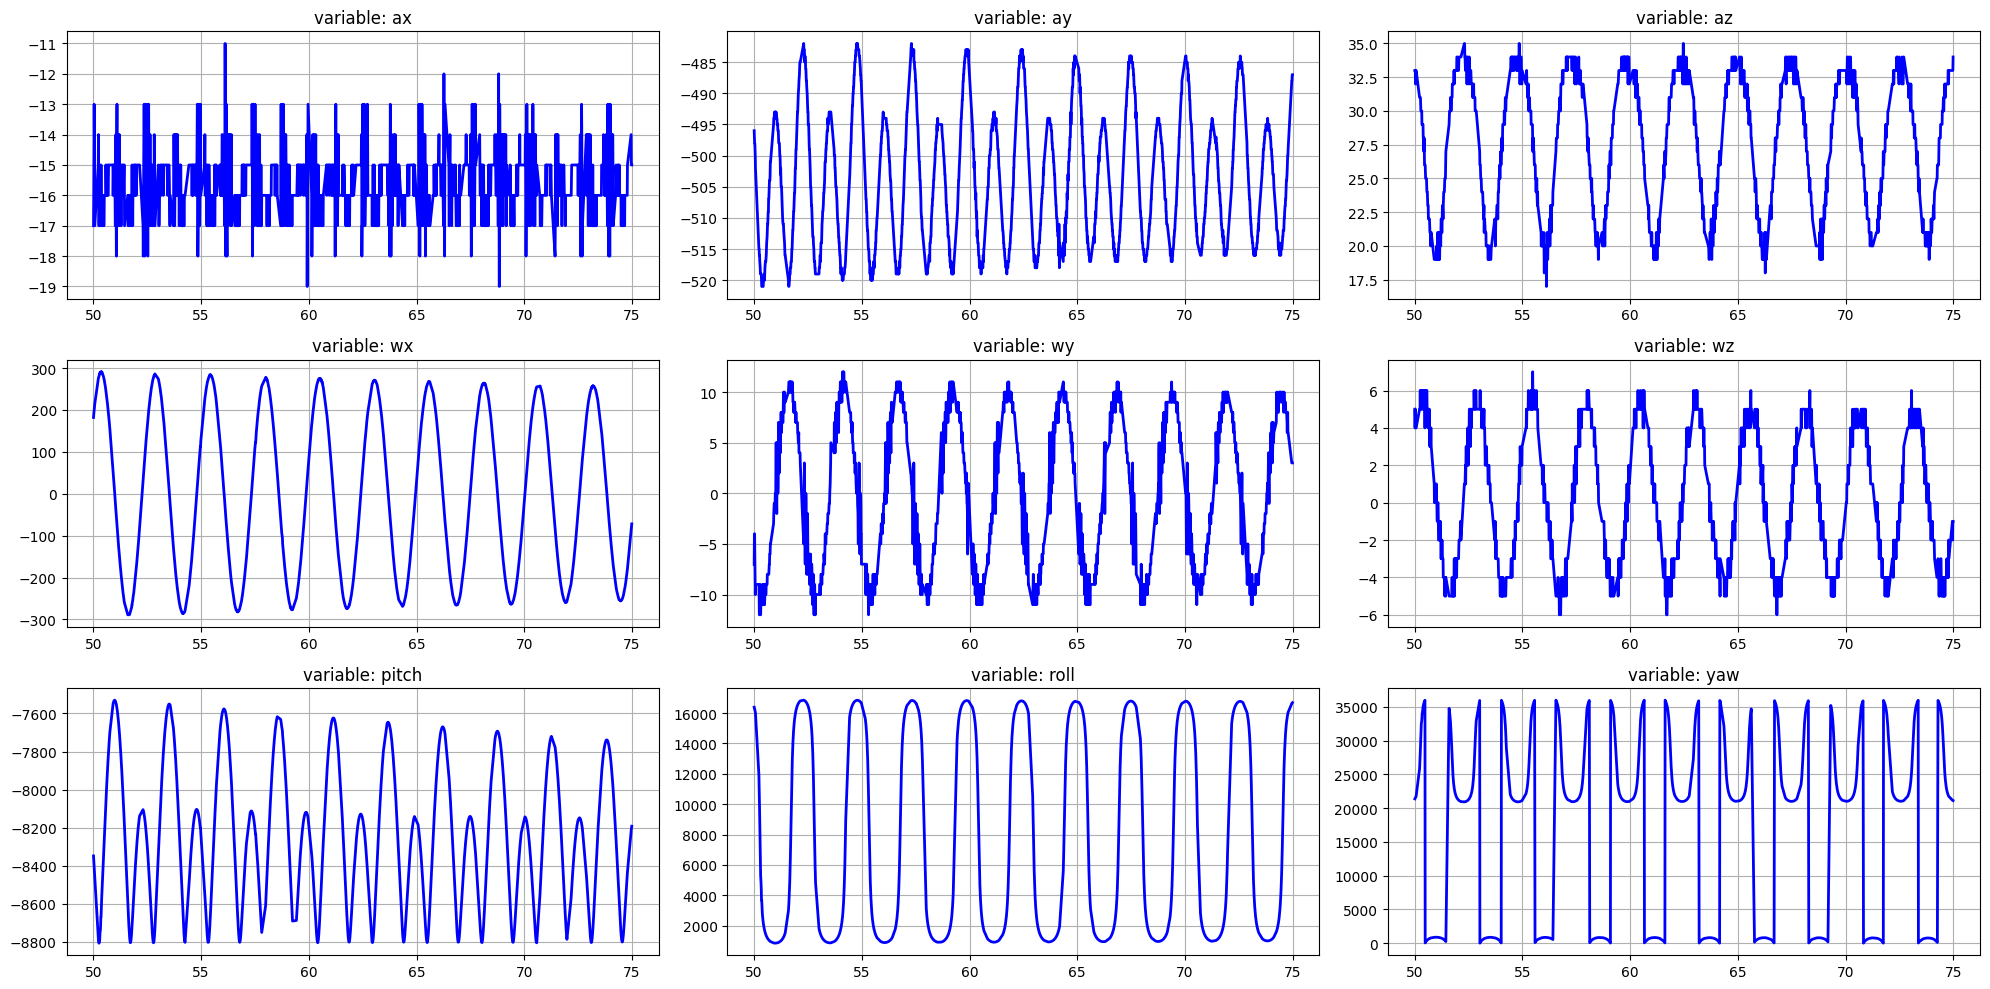
\includegraphics[width=\linewidth]{imagens/orientation.png}
            
            \label{fig:graphs}
            \textbf{Fonte:} Autoria Própria
        \end{figure}

        Esses dados já passaram pelos principais filtros embutidos no próprio sensor Kernel, o que é válido, uma vez que, antes de implementar os algoritmos pesados no microcontrolador, é necessário verificar se, de fato, o sensor, sozinho e com os seus algoritmos de filtragem e fusão, é capaz de obter as variáveis de interesse com a devida precisão e acurácia.

        Os primeiros gráficos brutos do sensor, em comparação com o encoder do pêndulo e ainda sem correções ou calibrações, podem ser evidenciados na figura subsequente, com os dados padronizados mostrando a variação angular no eixo x. A figura compara o pêndulo com o encoder, que de fato se mostram similares. Observa-se a similaridade das curvas e a confirmação de que esta medição obedece ao comportamento ideal do sistema.
        
        \begin{figure}[H]
            \centering
            \caption{Comparação do Encoder com o DRMM}
            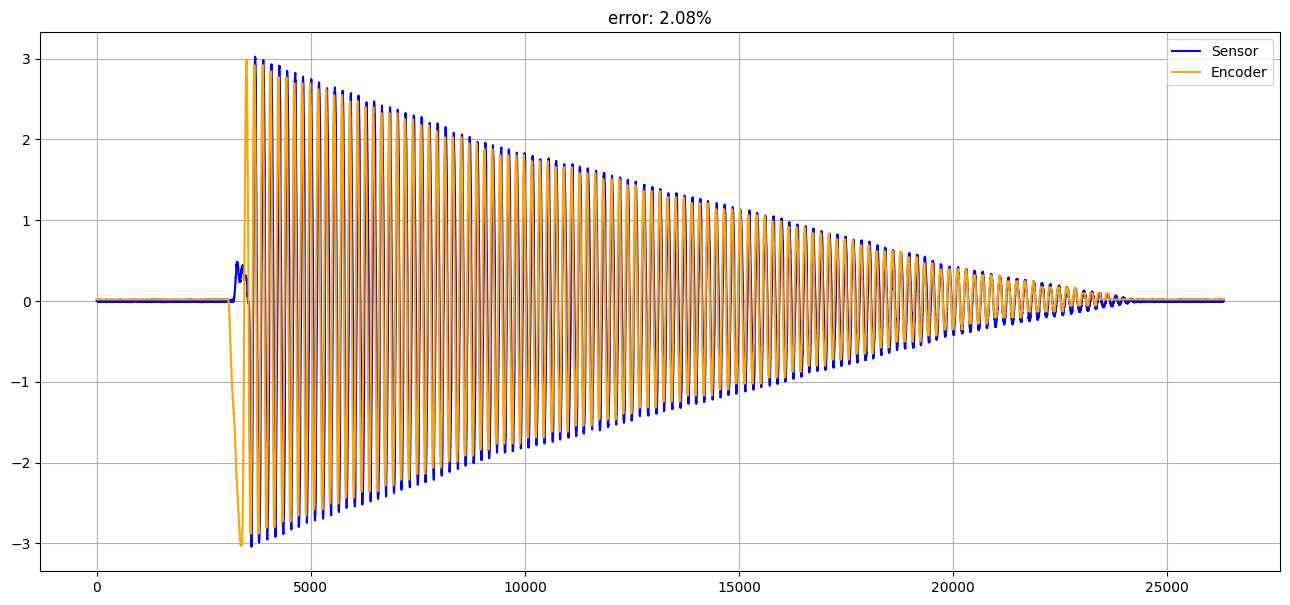
\includegraphics[width=.75\linewidth]{imagens/modelling.png}
            
            \label{fig:diagrama}
            \textbf{Fonte:} Autoria Própria
        \end{figure}

        O comportamento oscilatório é de fato capturado pelo sensor e pode ser corrigido para a mesma escala de acordo com o comprimento do pêndulo (regime estacionário). Observa-se que o atrito atua diretamente ao reduzir a amplitude da forma senoidal até estabilizar e se tornar estático (regime permanente) \cite{frank_angelo_pacala_b56d08da}. A \autoref{fig:graf4} já utiliza uma aproximação linear para o ajuste das variáveis em um encoder simples, onde já se observa avanço notável a partir da métrica R2 Score.

        \begin{figure}[H]
            \centering
            \caption{Comparação do Encoder com o DRMM (Ajuste Linear)}
            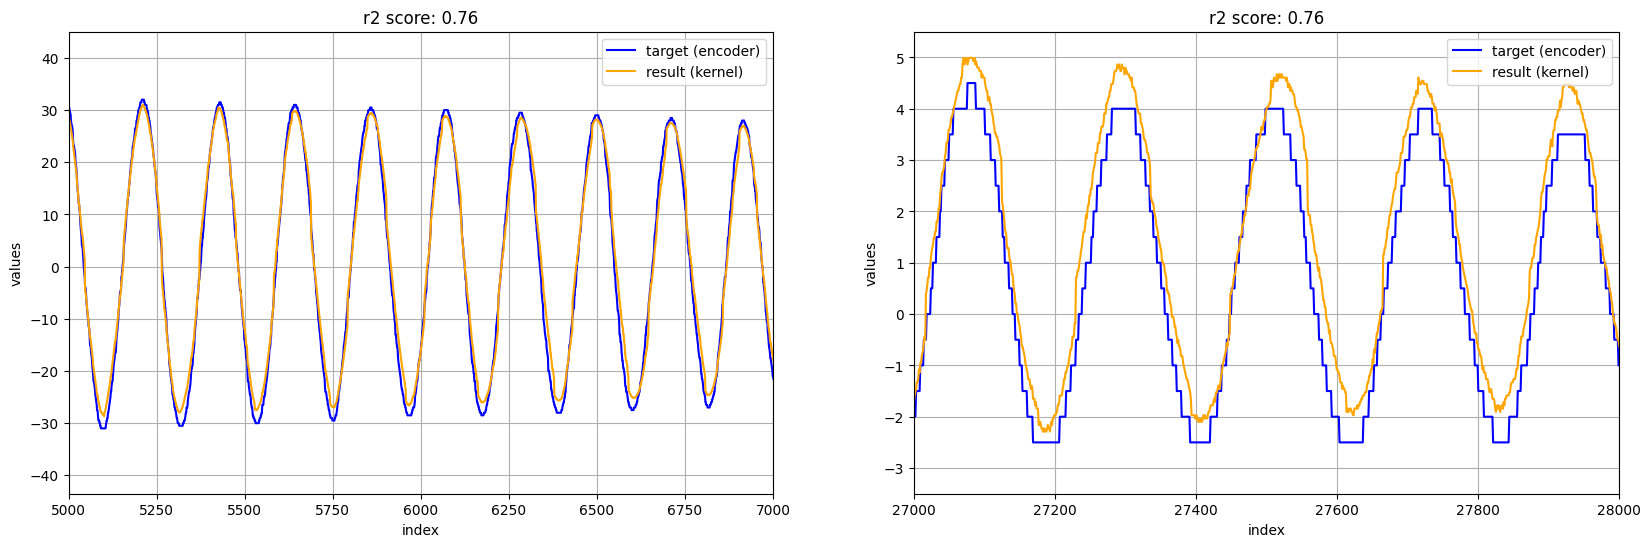
\includegraphics[width=.95\linewidth]{imagens/graf4.png}
            
            \label{fig:graf4}
            \textbf{Fonte:} Autoria Própria
        \end{figure}

        Observa-se que, ao ampliar a visualização (zoom) a partir do momento em que a amplitude das oscilações começa a diminuir, percebe-se que o sensor Kernel apresenta um nível de suavização e precisão muito superior ao do encoder, o qual exibe degraus discretos característicos de sua resolução limitada e quantização. Essa limitação do encoder atual compromete sua função como referência confiável para calibração, evidenciando a necessidade imperativa de adquirir um modelo mais preciso (já adquirido e a ser testado), capaz de gerar dados de referência superiores aos do sensor para validar e otimizar os algoritmos de calibração de forma robusta.
            
\newpage
\section{Considerações Finais}
    Nesta macroentrega, foram alcançados avanços significativos no desenvolvimento do Dispositivo de Referência de Monitoramento dos Movimentos, incluindo a integração de um processador ESP32-S3 com sensor Kernel Motion Sensor AHRS em uma placa de circuito impresso personalizada e embalagem protetora impressa em 3D, com massa otimizada de 451,6 g. Os testes de bancada validaram a transmissão de dados em até 100 Hz via USB, RS422 ou Wi-Fi com Protocol Buffers para serialização eficiente, enquanto a montagem do pêndulo simples, inspirado em aparatos para comparação de IMUs, permitiu oscilações controladas em 2 eixos com encoder angular para referência. 
    
    Os testes estáticos e dinâmicos demonstraram a captura precisa do comportamento oscilatório pelo sensor, com curvas similares às do encoder, confirmando a eficácia inicial dos filtros embarcados antes de calibrações adicionais. No entanto, percebe-se pelos gráficos apresentados que o encoder do experimento não atingiu uma precisão superior a do sensor Kernel, impossibilitando uma calibração confiável e robusta e evidenciando a necessidade de se um adquirir um mais preciso que ja foi comprado e será testado assim que chegar.

    Por fim, é importante destacar que haverá o aluguel de um dispositivo de movimento concorrente, que servirá como padrão de referência para comparações após a calibração do protótipo. Dessa forma, será possível avaliar se a calibração atende aos requisitos de um concorrente e aos padrões gerais demandados pelo mercado para este tipo de aplicação, concluindo o ciclo de prototipagem do projeto e avançando para a fase comercial.
    
\newpage
\bibliography{references}
\end{document}